\documentclass[10pt,pdf,aspectratio=169,hyperref={unicode}]{beamer}

\usepackage[T2A]{fontenc}
\usepackage[utf8]{inputenc}
\usepackage[english,russian]{babel}
\usepackage{amssymb,amsfonts,amsmath}
\usepackage{graphicx}
\usepackage[font=small,skip=0pt]{caption}

\captionsetup[table]{font=small,skip=5pt}

\let\Tiny=\tiny

\setbeamertemplate{caption}[numbered]
\setbeamertemplate{theorems}[numbered]
\setbeamertemplate{navigation symbols}{}
\setbeamerfont{caption}{size=\footnotesize}

\definecolor{links}{HTML}{2A1B81}
\hypersetup{colorlinks,linkcolor=,urlcolor=links}

\usetheme{Pittsburgh}
\usecolortheme{whale}

\let\Definition\relax
\newtheorem{Definition}{Определение}
\let\Theorem\relax
\newtheorem{Theorem}{Теорема}

\newcommand{\inp}[1]{\input{../../out/#1}}
\newcommand{\characteristic}[2]{\inp{#1/characteristics/#2}}
\newcommand{\descriptive}[2]{\inp{#1/descriptive/#2}}
\newcommand{\test}[3]{\inp{#1/test/#2/#3}}
\newcommand{\normaldistr}{$\mathcal{N}(\descriptive{original}{mean}, \descriptive{original}{variance})$}
\newcommand{\resnormaldistr}{$\mathcal{N}(\descriptive{residual}{mean}, \descriptive{residual}{variance})$}

\logo{
\includegraphics[width=1cm,height=1cm,keepaspectratio]{Logo_BSU.jpg}}

\title{Анализ и прогнозирование гидрологических данных}
\subtitle[]{}
\author[Павлов Александр \hspace{0.2\textwidth} \insertframenumber\,/\,\inserttotalframenumber]{ Павлов Александр Сергеевич \\ \vspace{2em} \small{Научный руководитель: Цеховая Татьяна Вячеславовна \\Рецензент: Рафеенко Екатерина Дмитриевна} }

\institute[]{Кафедра Теории Вероятностей и Математической Статистики \vspace{2pt} \\ Факультет Прикладной Математики и Информатики \vspace{2pt} \\ Белорусский Государственный Университет }
\date{Минск, 2015}

\begin{document}

\begin{frame}[plain]
  \titlepage
\end{frame}

\section[Содержание]{}
\begin{frame}
  \frametitle{Содержание}
  \tableofcontents
\end{frame}

\section{Обзор реализованного программного обеспечения}

\begin{frame}
  \frametitle{Особенности}
  \begin{itemize}
    \item Доступно с любого устройства, имеющего доступ в интернет, по адресу \href{https://apaulau.shinyapps.io/batorino}{apaulau.shinyapps.io/batorino}
    \item Реализовано на языке программирования \textbf{R}
    \item Логически разделёно на три модуля
    \item Имеет простой, быстро расширяемый гибкий интерфейс
    \item Широкие графические возможности
    \item Проверка тестов и критериев
    \item Мгновенный отклик на изменение параметров
    \item Быстрая проверка различных моделей
  \end{itemize}
\end{frame}

\subsection{Модуль предварительного анализа}

\begin{frame}
  % \frametitle{Первичный анализ и описательные статистики}
  \frametitle{Модуль предварительного анализа}
    \begin{figure}[h]
    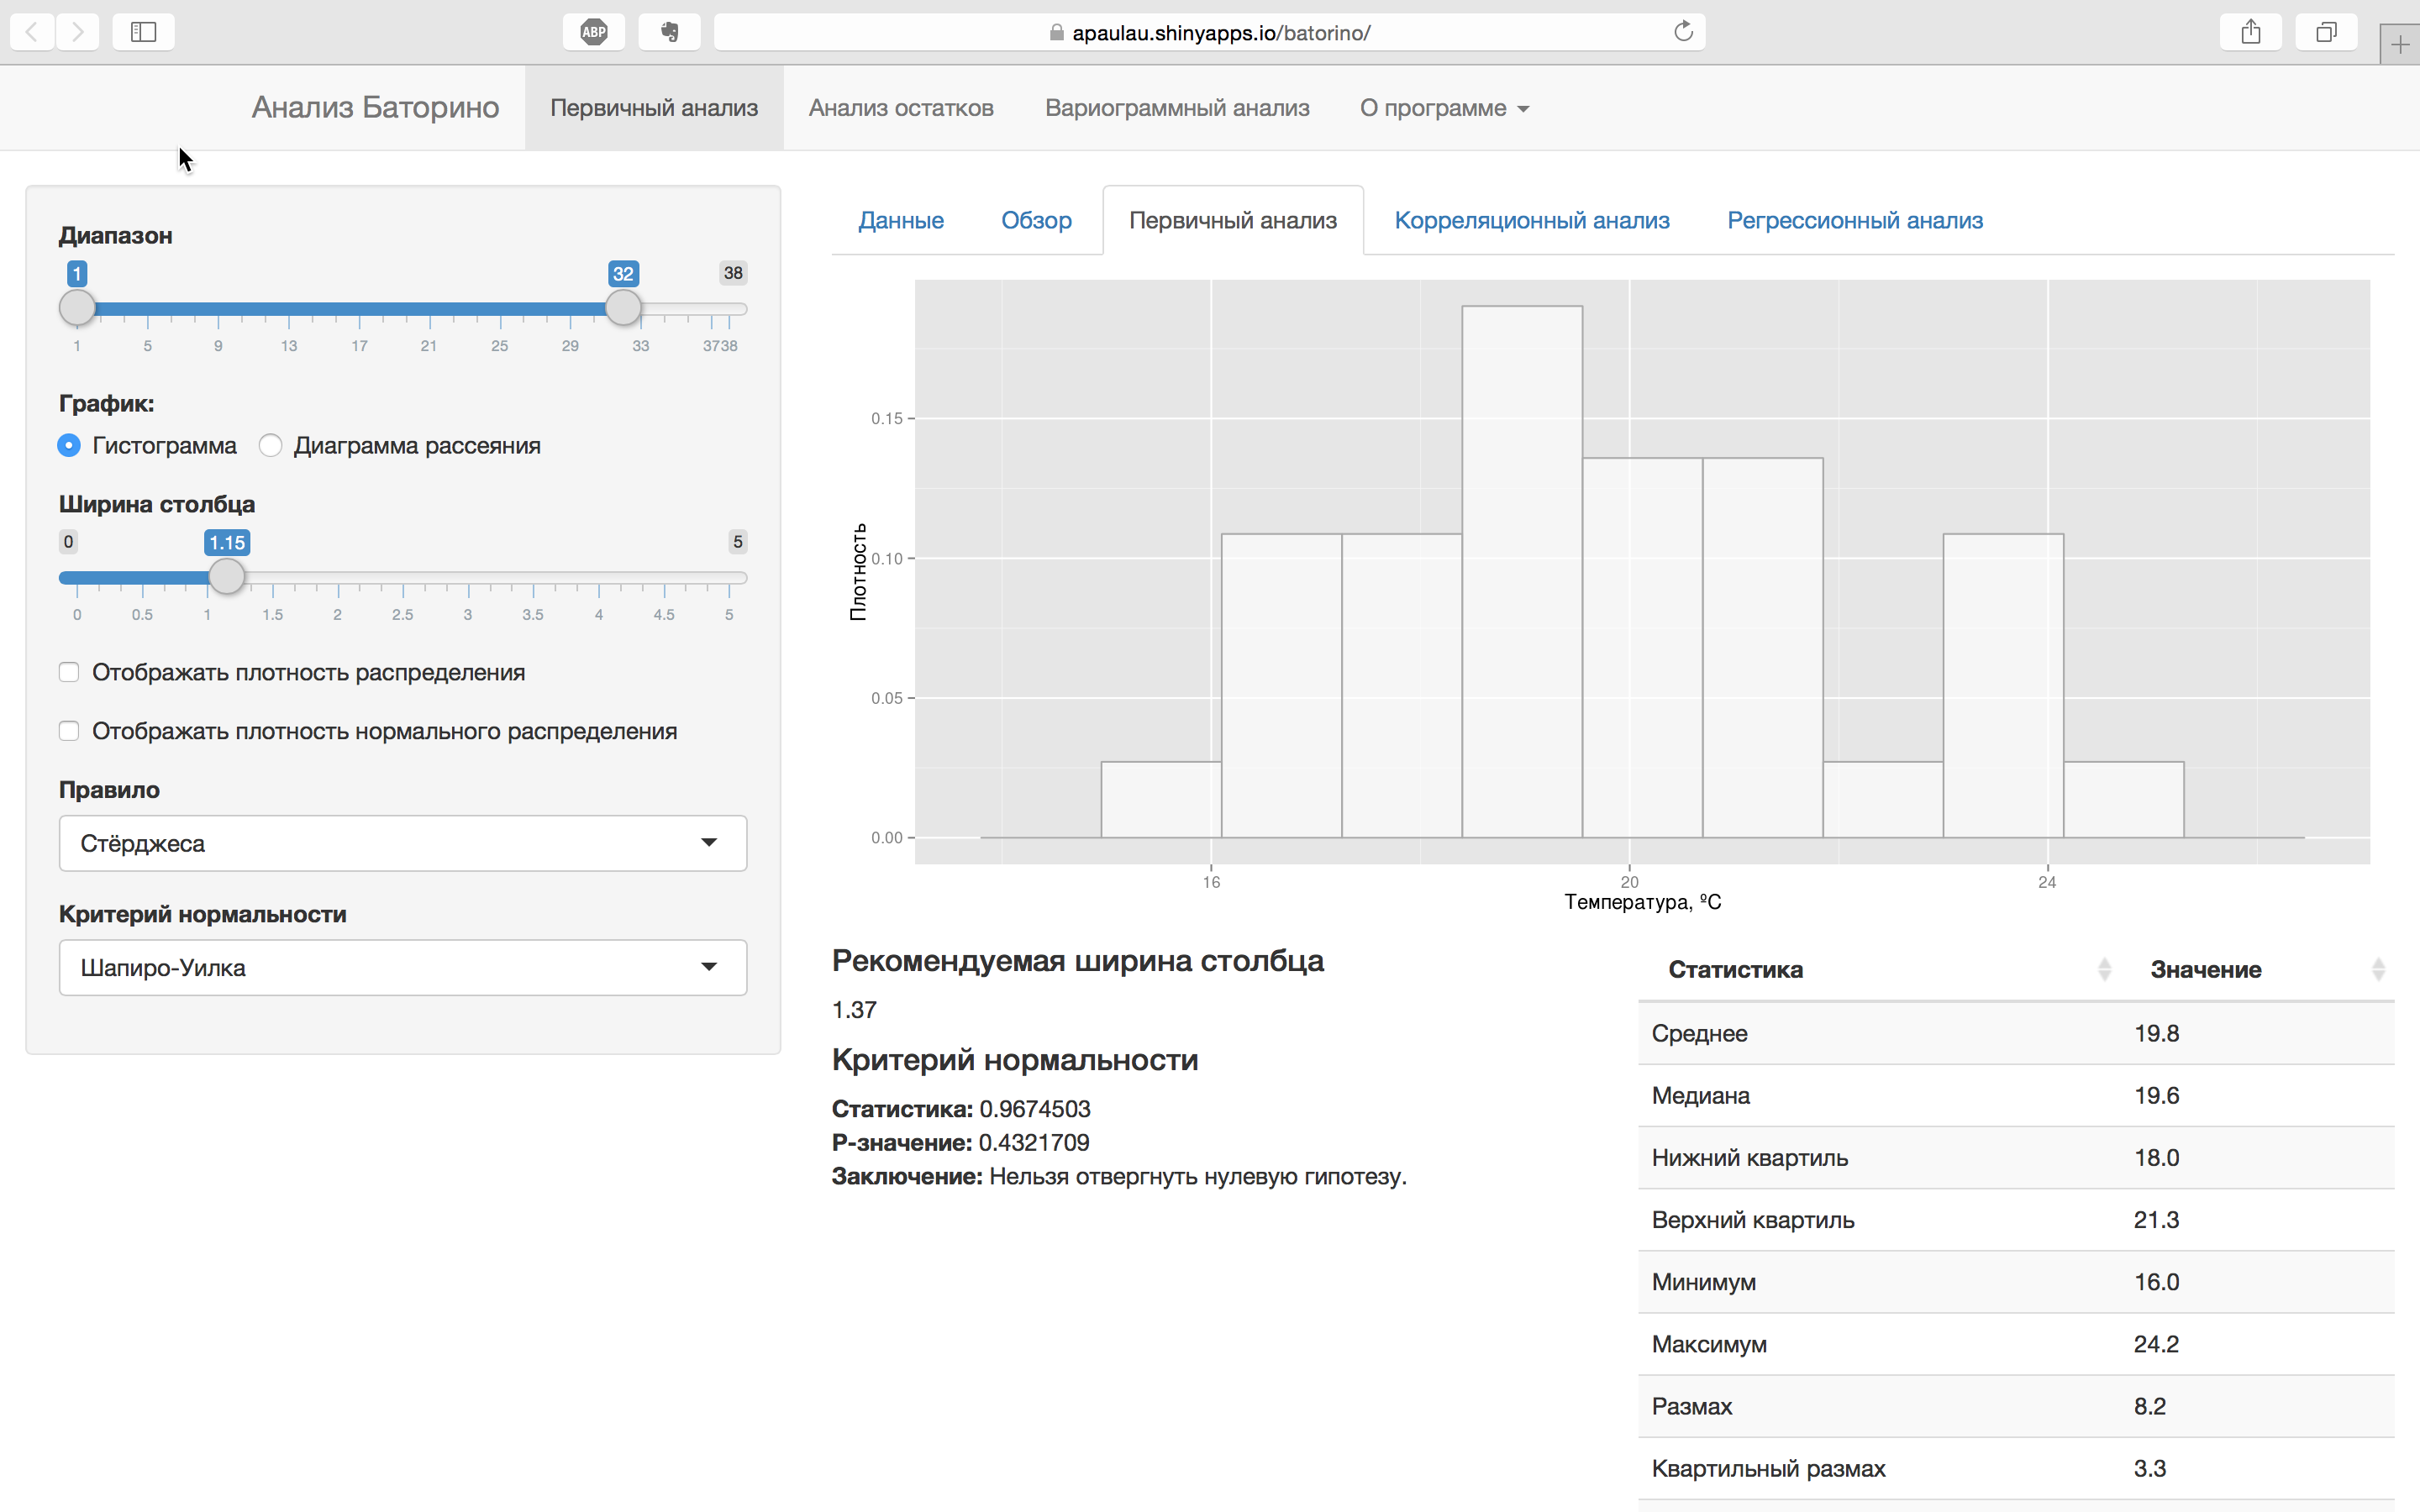
\includegraphics[width=0.75\textwidth]{../../figures/static/1_basis.png}
    \caption{Первичный анализ и описательные статистики}
  \end{figure}
\end{frame}

\begin{frame}
  % \frametitle{Корреляционный анализ}
  \frametitle{Модуль предварительного анализа}
  \begin{figure}[h]
    \center{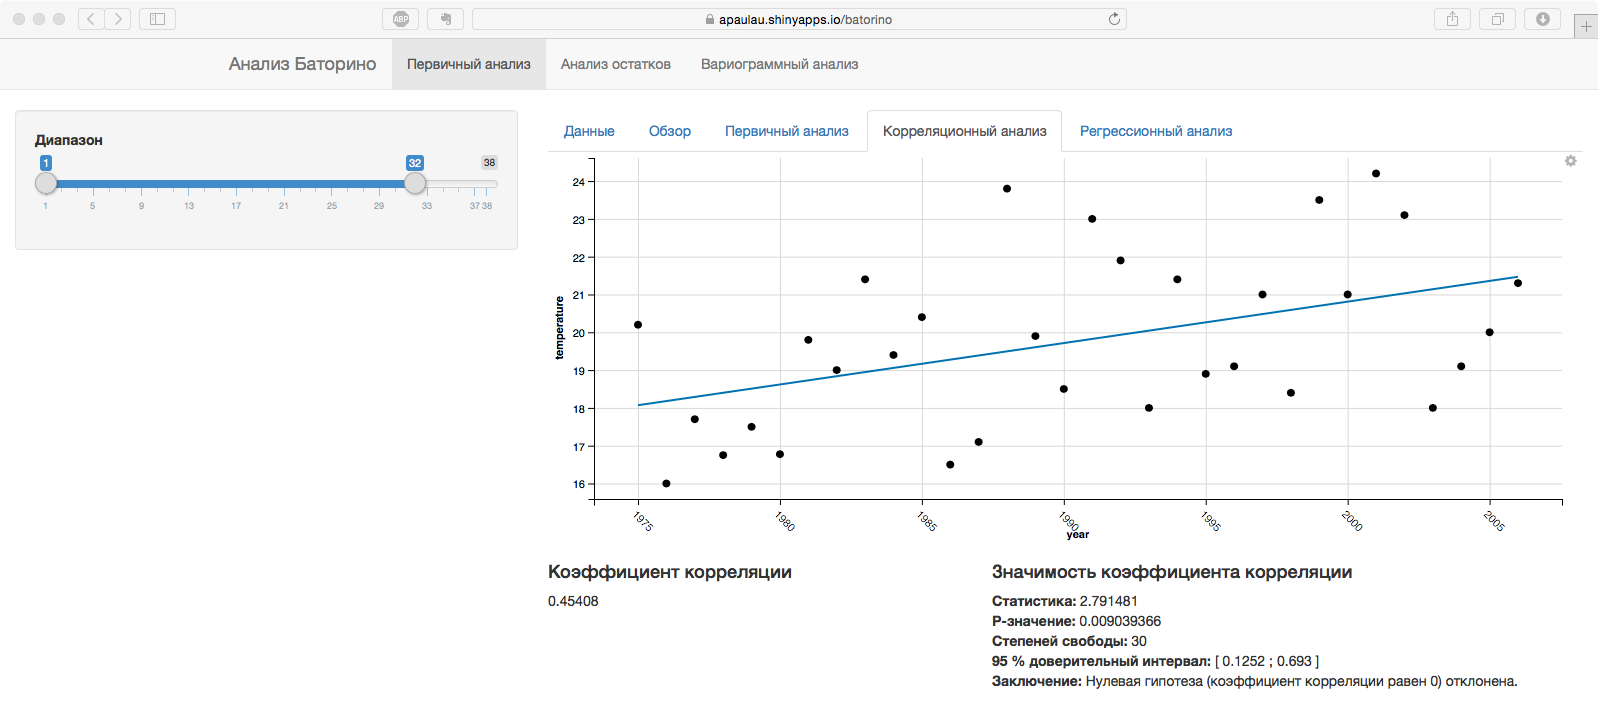
\includegraphics[width=0.75\textwidth]{../../figures/static/p_corr.png}}
    \caption{Корреляционный анализ}
  \end{figure}
\end{frame}

\begin{frame}
  % \frametitle{Регрессионный анализ}
  \frametitle{Модуль предварительного анализа}
    \begin{figure}[h]
    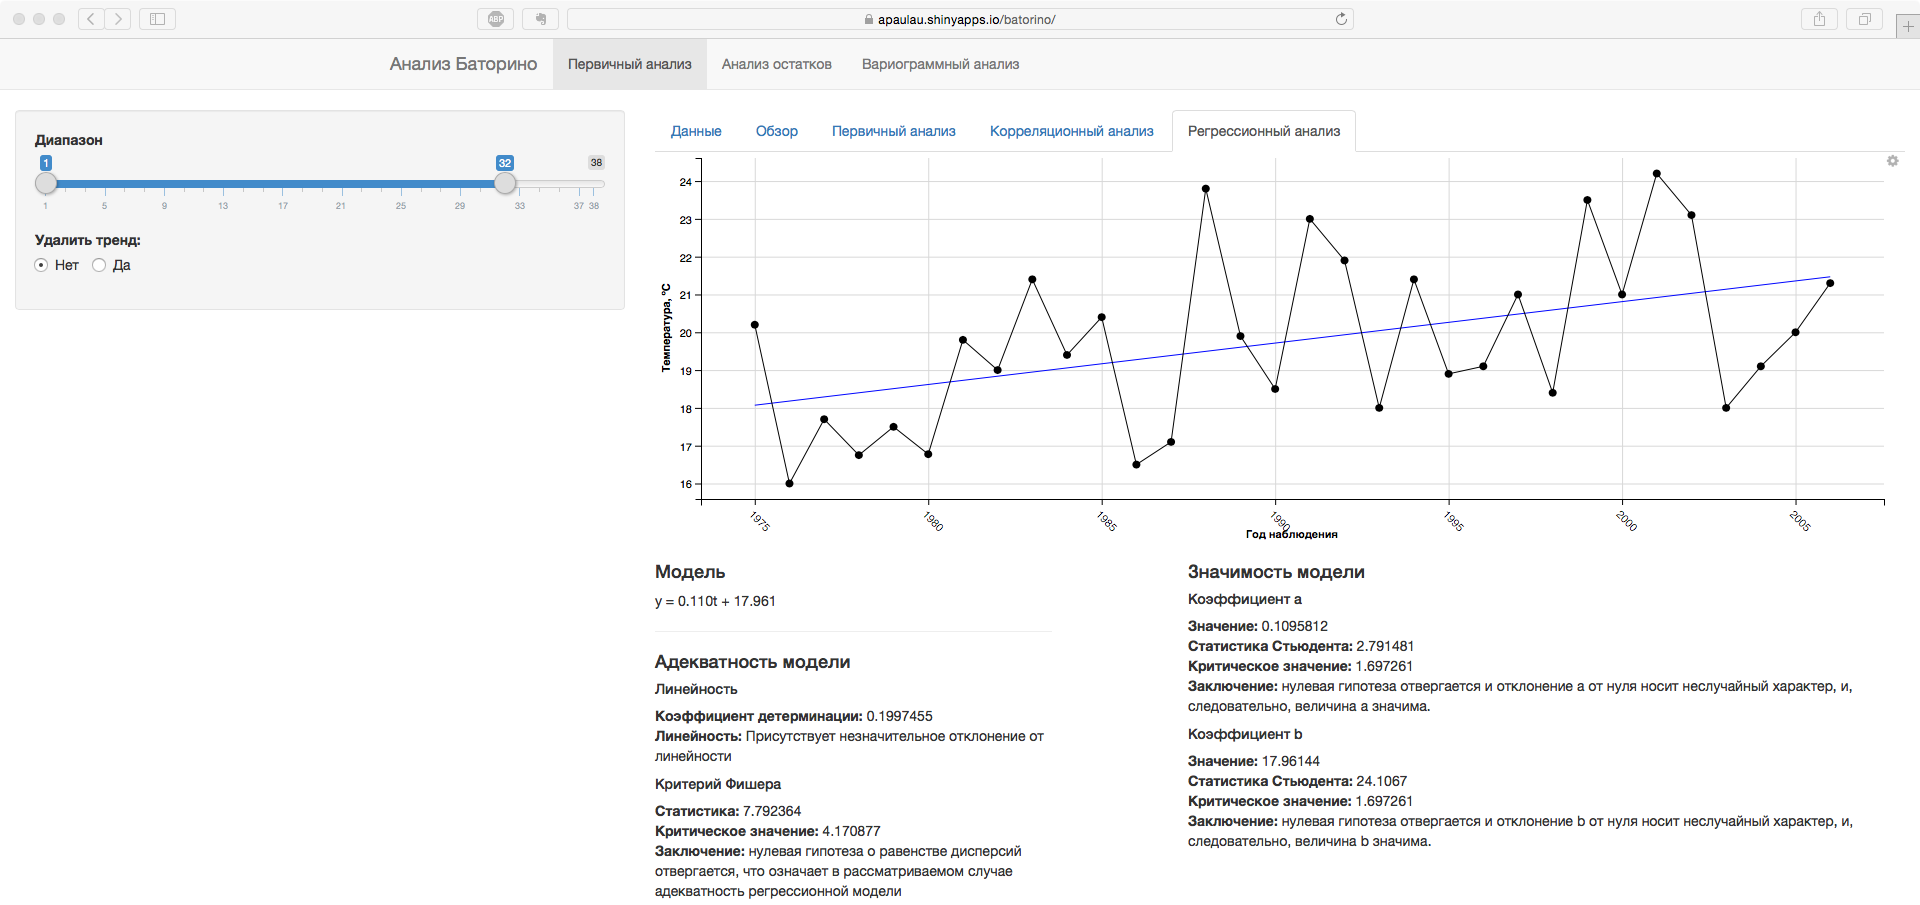
\includegraphics[width=0.75\textwidth]{../../figures/static/2_regr.png}
    \caption{Регрессионный анализ}
  \end{figure}
\end{frame}

\subsection{Модуль анализа остатков}

\begin{frame}
  % \frametitle{Автокорреляционная функция}
  \frametitle{Модуль анализа остатков}
    \begin{figure}[h]
    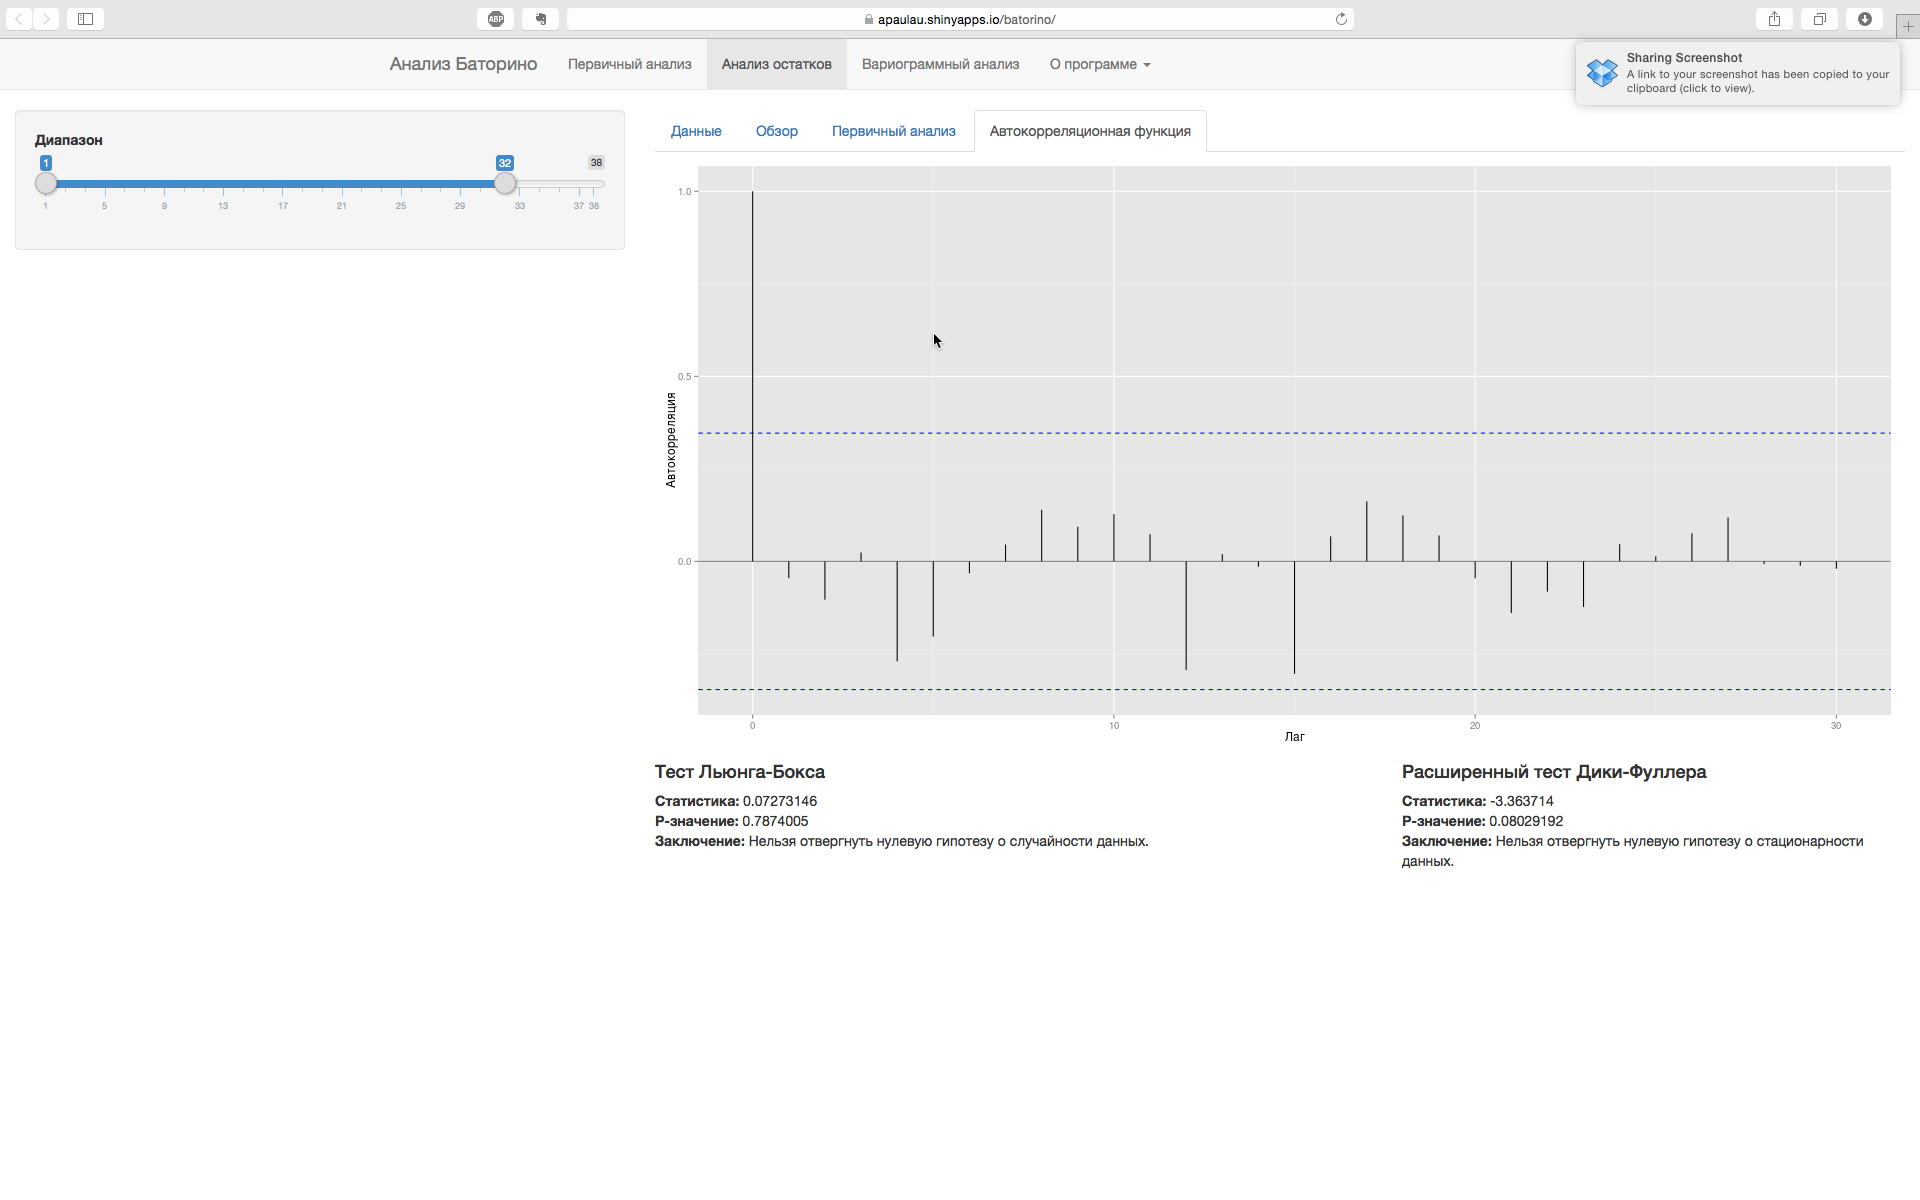
\includegraphics[width=0.75\textwidth]{../../figures/static/3_acf.png}
    \caption{Автокорреляционная функция}
  \end{figure}
\end{frame}

\subsection{Модуль вариограммного анализа}

\begin{frame}
  % \frametitle{Возможности по подбору модели вариограммы}
  \frametitle{Модуль вариограммного анализа}
    \begin{figure}[h]
    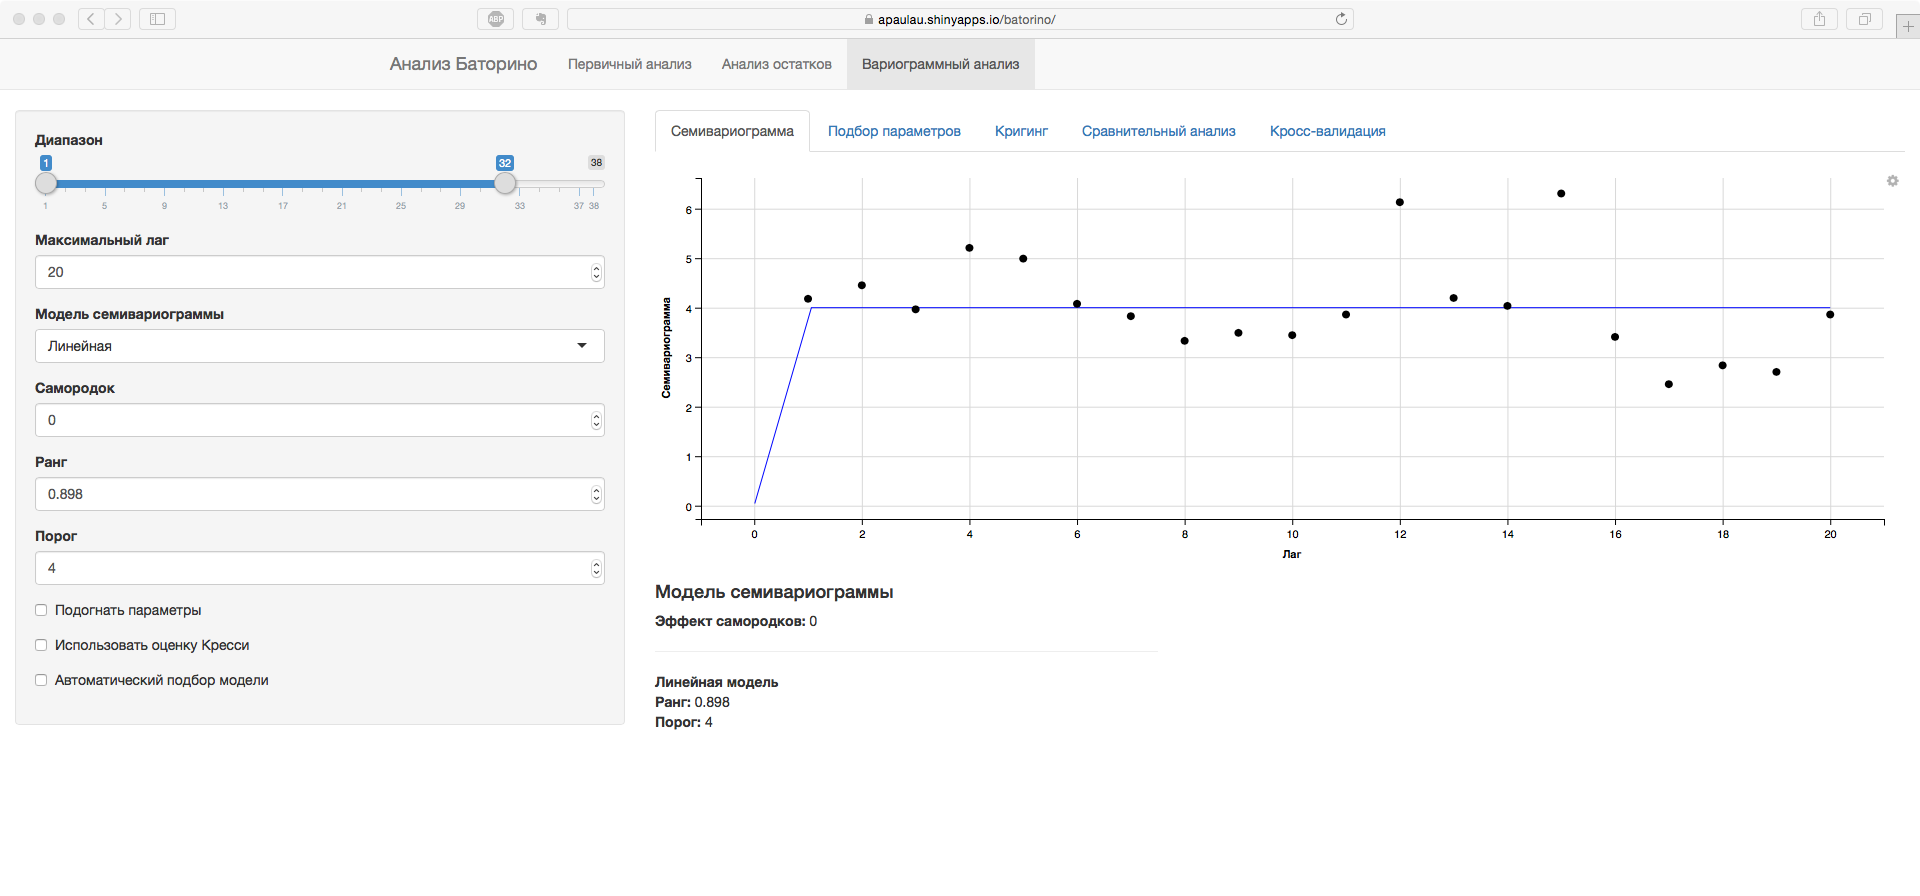
\includegraphics[width=0.75\textwidth]{../../figures/static/4_variogram.png}
    \caption{Возможности по подбору модели вариограммы}
  \end{figure}
\end{frame}

\begin{frame}
  % \frametitle{Подбор параметров модели вариограммы}
  \frametitle{Модуль вариограммного анализа}
    \begin{figure}[h]
    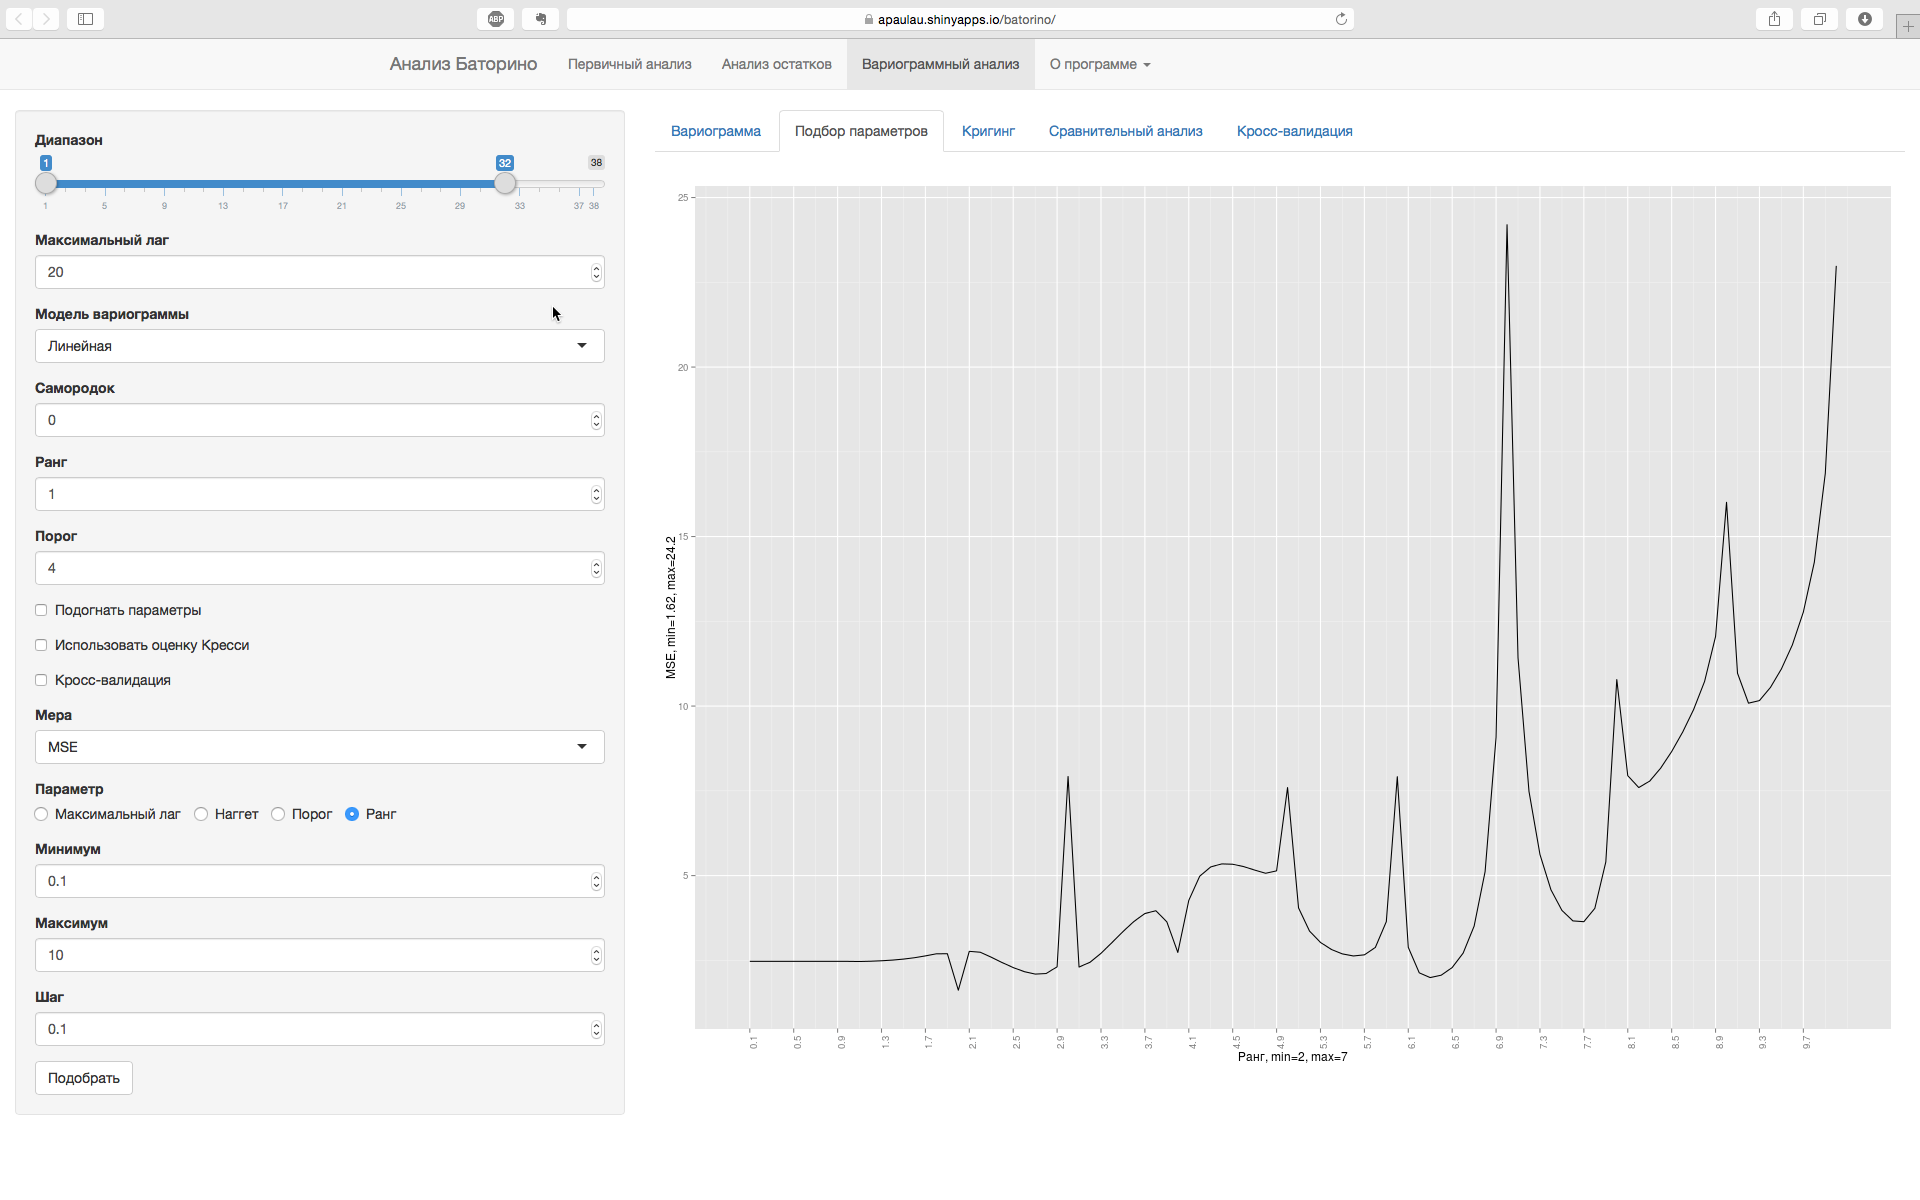
\includegraphics[width=0.75\textwidth]{../../figures/static/5_fit.png}
    \caption{Подбор параметров модели вариограммы}
  \end{figure}
\end{frame}

\begin{frame}
  % \frametitle{Сравнение прогнозных значений}
  \frametitle{Модуль вариограммного анализа}
    \begin{figure}[h]
    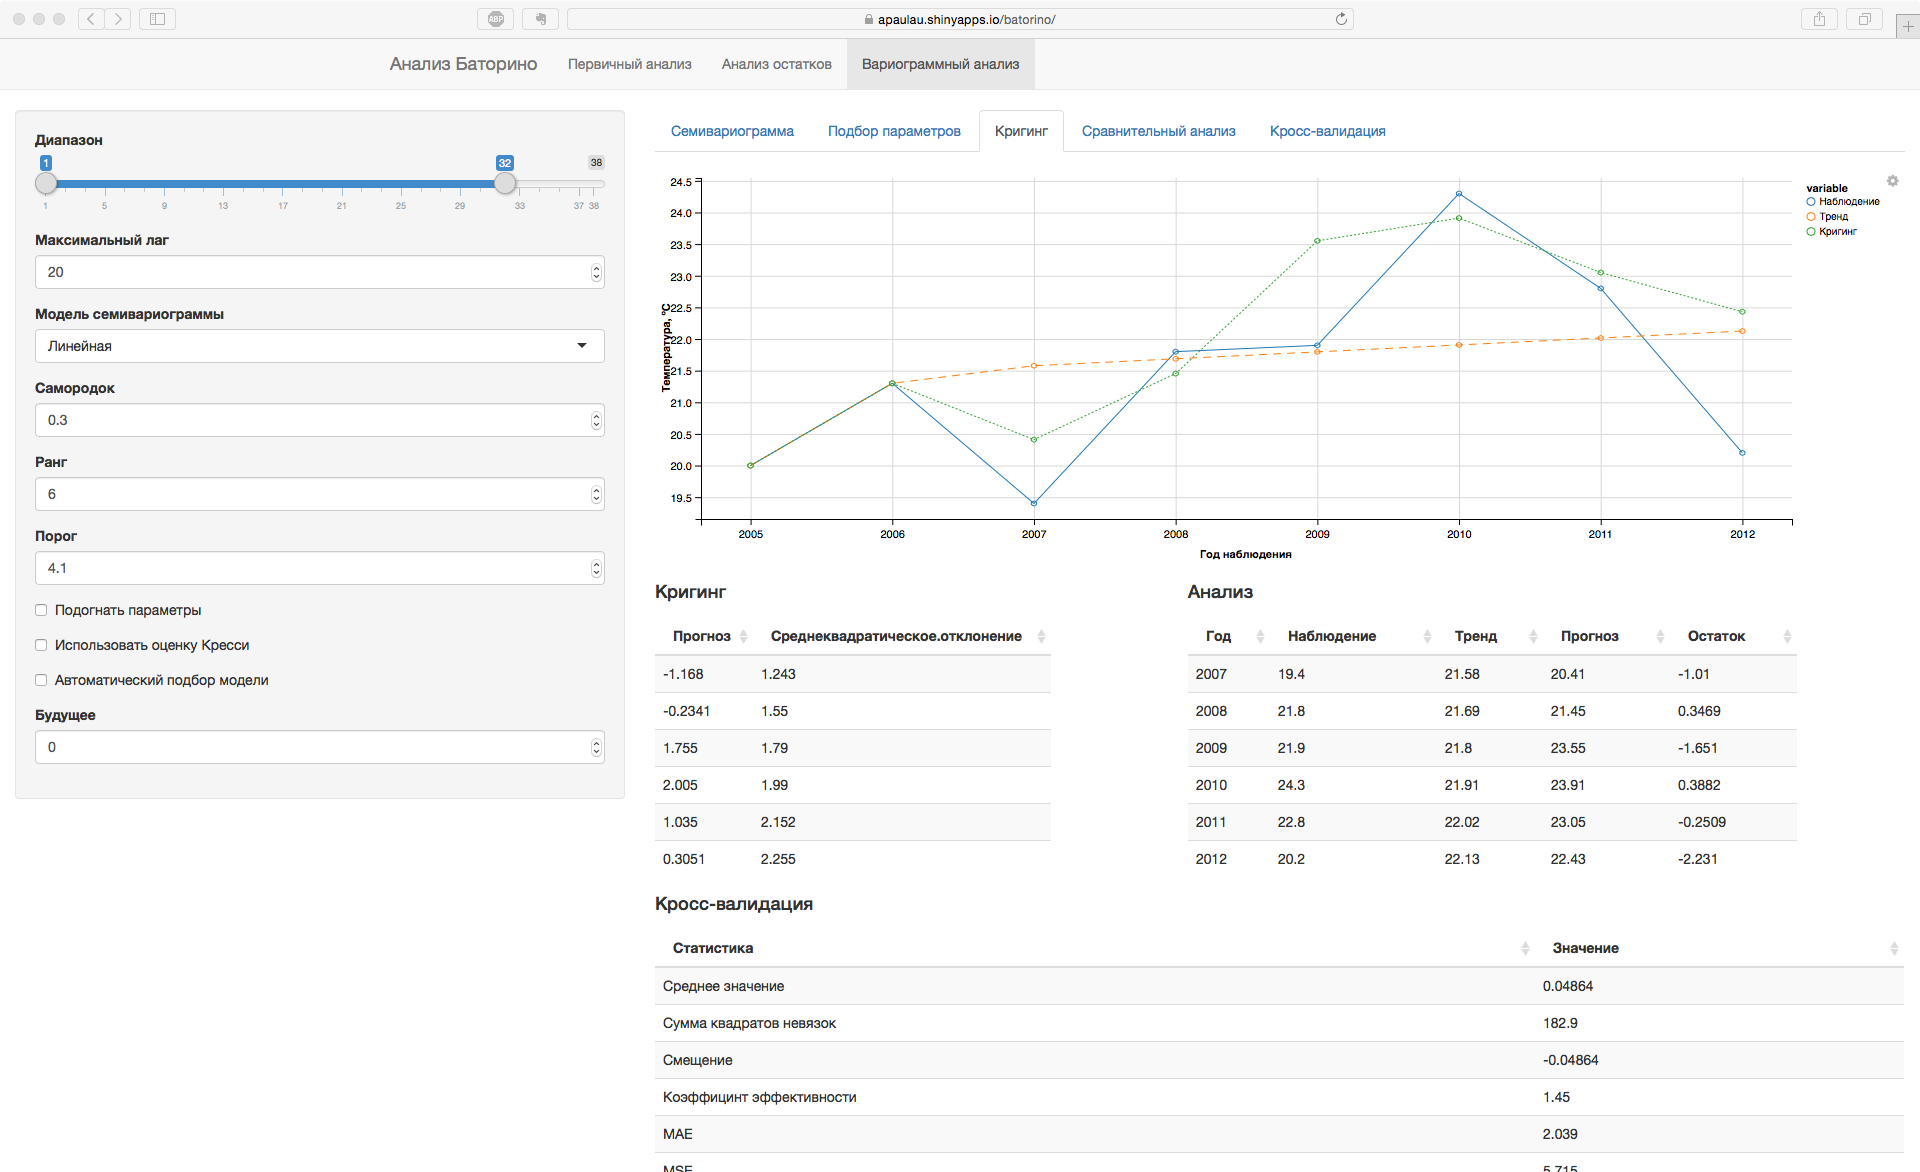
\includegraphics[width=0.75\textwidth]{../../figures/static/6_krige.png}
    \caption{Сравнение прогнозных значений}
  \end{figure}
\end{frame}

\section{Детерминированный подход}

\begin{frame}
  \frametitle{Исходные данные}
  \begin{columns}[c]
  \column{2in}
  Исседуемые данные получены от учебно-научного центра <<Нарочанская биологическая станция им. Г.Г.Винберга>>.

  \vspace{0.5em}

  Исходные данные представляют собой выборку $ X(t) $, состоящую из значений средней температуры воды в июле месяце каждый год в период с 1975 по 2012 годы.
  \column{4in}
  \begin{figure}[h]
    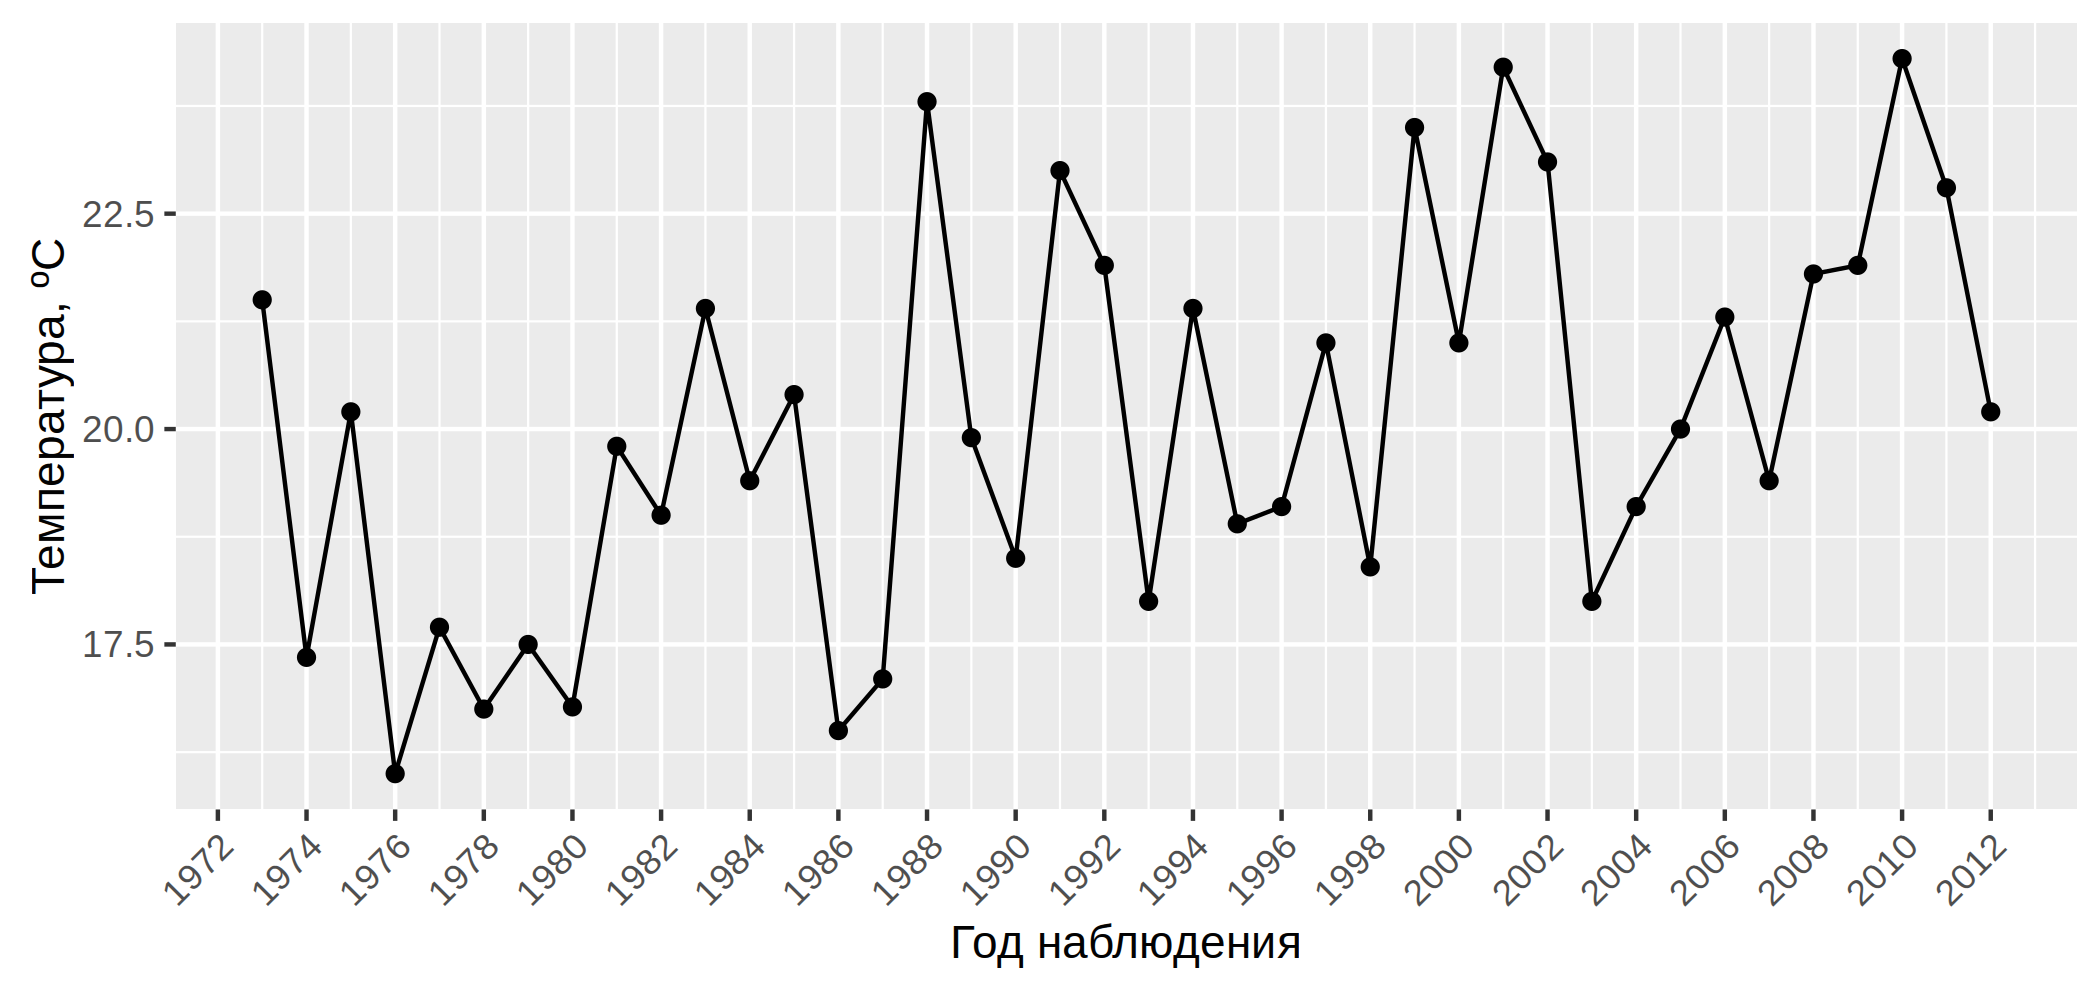
\includegraphics[width=1\linewidth]{../../figures/source.png}
    \caption{Исходные данные}
  \end{figure}
  \end{columns}
\end{frame}

\subsection{Проверка на нормальность}

\begin{frame}
  \frametitle{Проверка на нормальность}
  \begin{columns}[c]
  \column{2in}
  Визуально и проверкой критериев Шапиро-Уилка, $\chi^2$-Пирсона и Колмогороваа-Смирнова была показана близость выборочного распределения к нормальному с параметрами \normaldistr.

  \vspace{0.5em}

  При этом выборочное распредлеение характеризуется небольшой скошенностью вправо (коэффициент асимметрии $ \descriptive{original}{skew} $) и пологостью пика кривой распределения ($ \descriptive{original}{kurtosis} $) относительного нормального.
  \column{4in}
  \begin{figure}[h]
    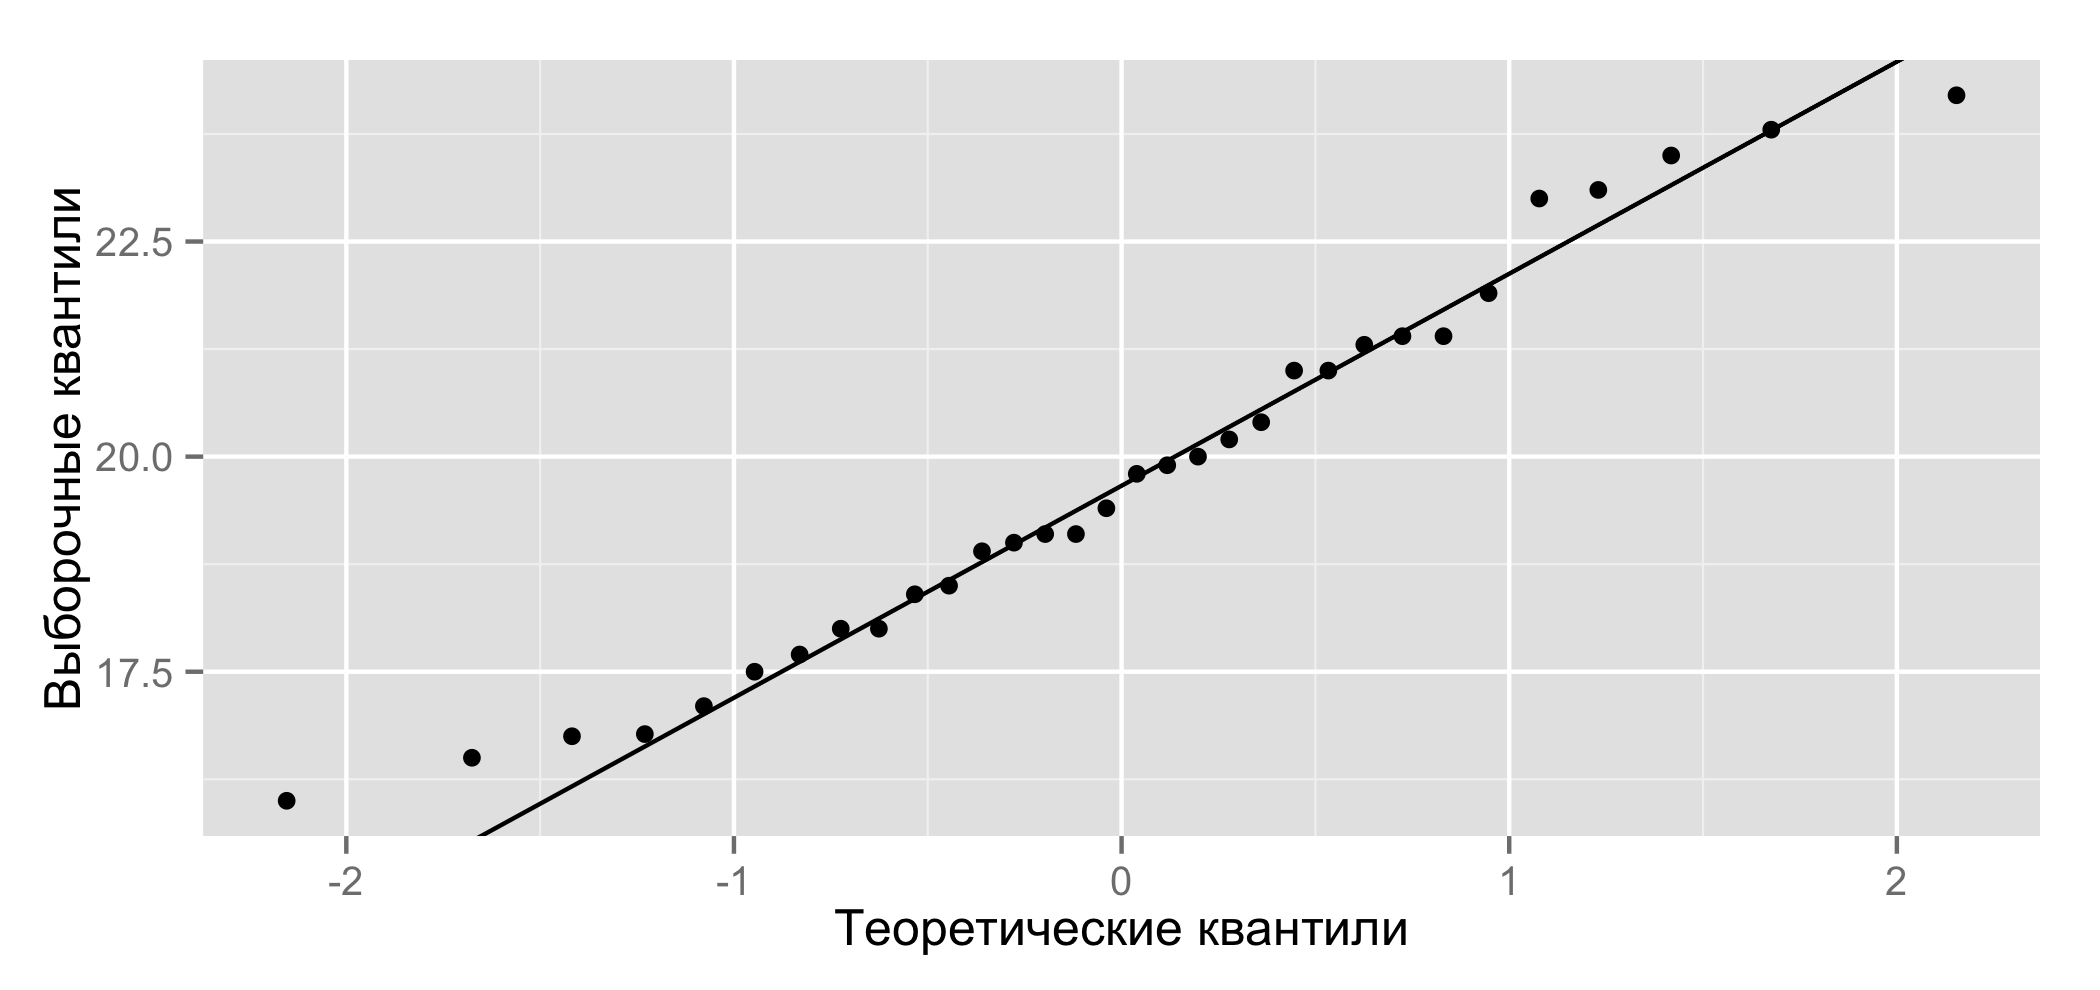
\includegraphics[width=1\linewidth]{../../figures/original/quantile.png}
    \caption{График квантилей}
  \end{figure}
  \end{columns}
\end{frame}

\subsection{Корреляционный анализ}

\begin{frame}
  \frametitle{Корреляционный анализ}
  \begin{columns}[c]
  \column{2in}
  С помощью критерия Граббса показано отсутствие выбросов в исходных данных.

  \vspace{0.5em}

  Вычислен выборочный коэффициент корреляции: $ r_{xt} = \characteristic{original}{correlation} $.

  \vspace{0.5em}

  При уровне значимости $ \alpha=0.05 $ доказана его значимость.
  \column{4in}
    \begin{figure}[h]
    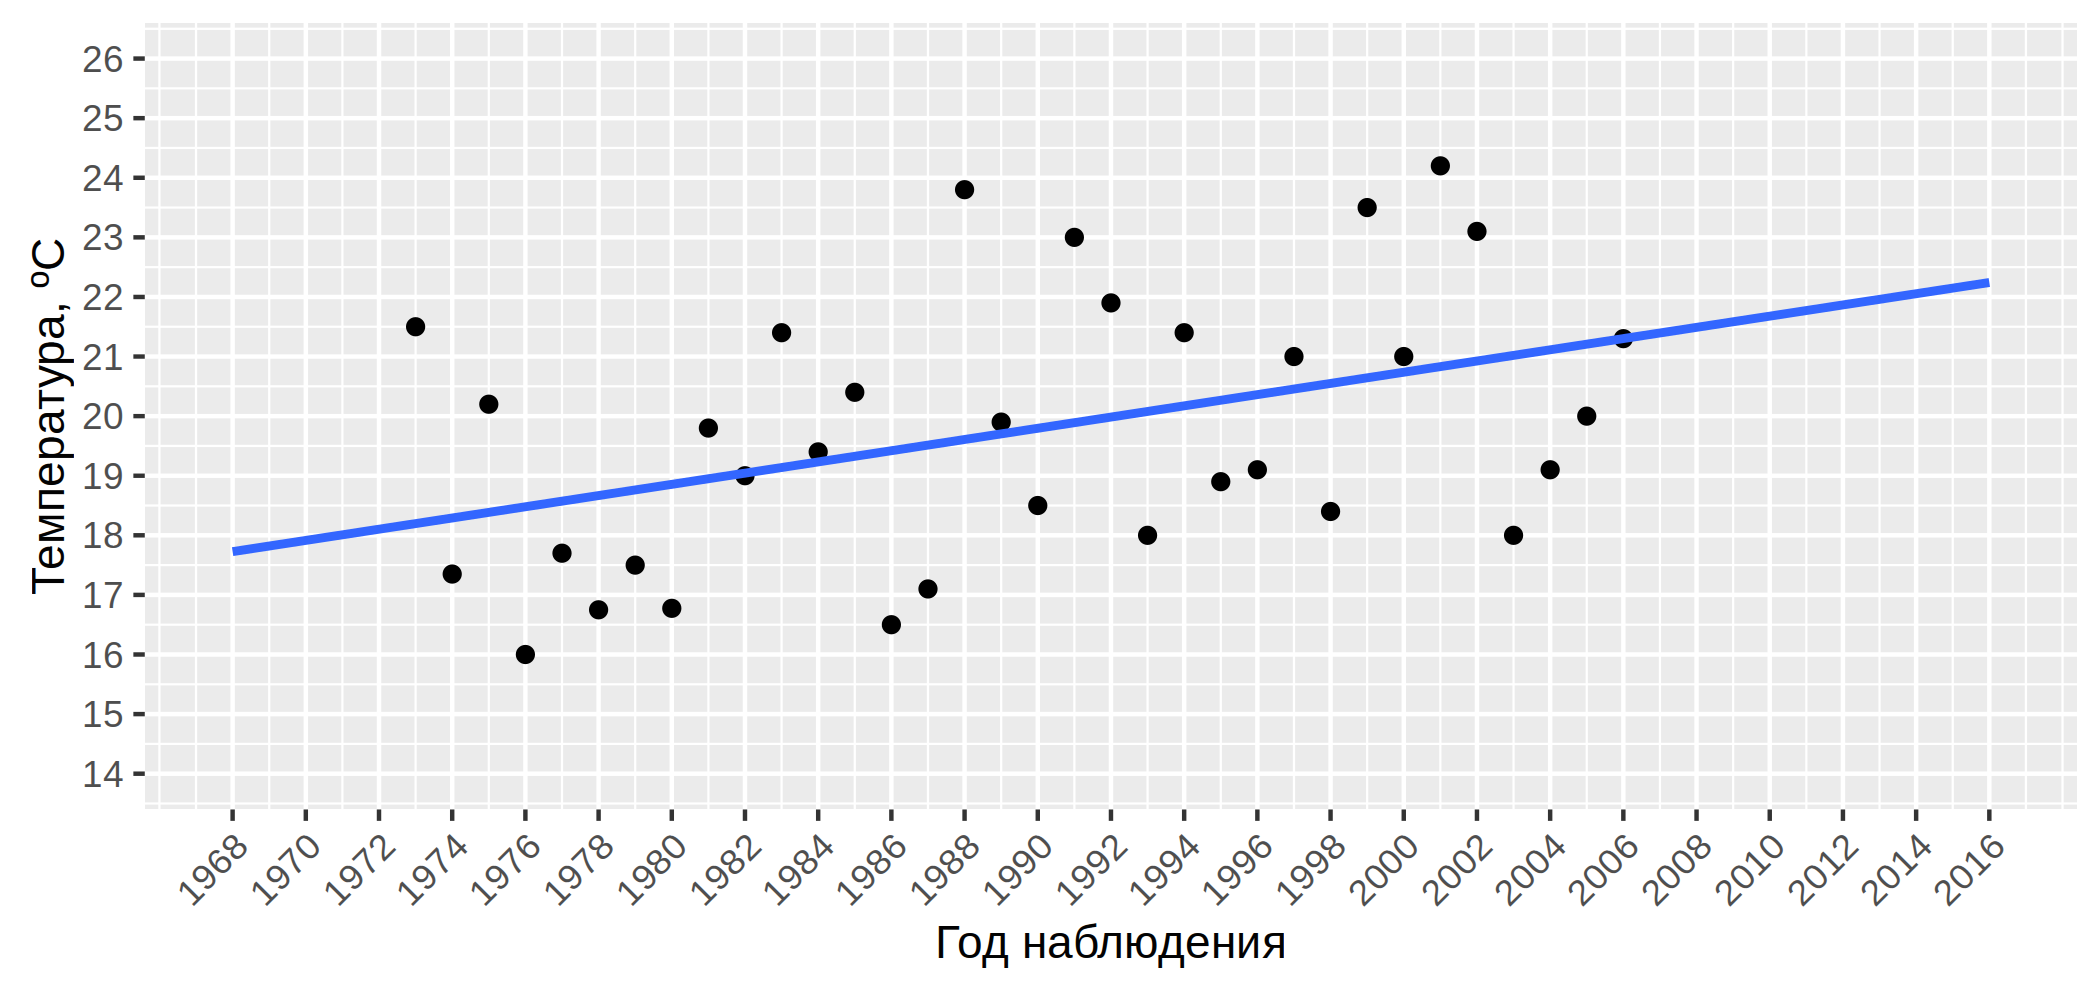
\includegraphics[width=1\linewidth]{../../figures/original/scatterplot.png}
    \caption{Диаграмма рассеяния}
  \end{figure}
  \end{columns}
\end{frame}

\subsection{Регрессионный анализ}

\subsubsection{Регрессионная модель}
\begin{frame}
  \frametitle{Регрессионная модель}
  \begin{columns}[c]
  \column{2in}
  Выявлено, что исследуемый временной ряд является аддитивным:
  \begin{equation}
    X(t) = y(t) + \varepsilon(t),
  \end{equation}
  где $ y(t) $ --- тренд, $ \varepsilon(t) $ --- нерегулярная составляющая.

  \vspace{0.5em}

  Найдена модель тренда: $ y(t) = at + b = 0.1014t + 18.0521 $
  \column{4in}
    \begin{figure}[h]
    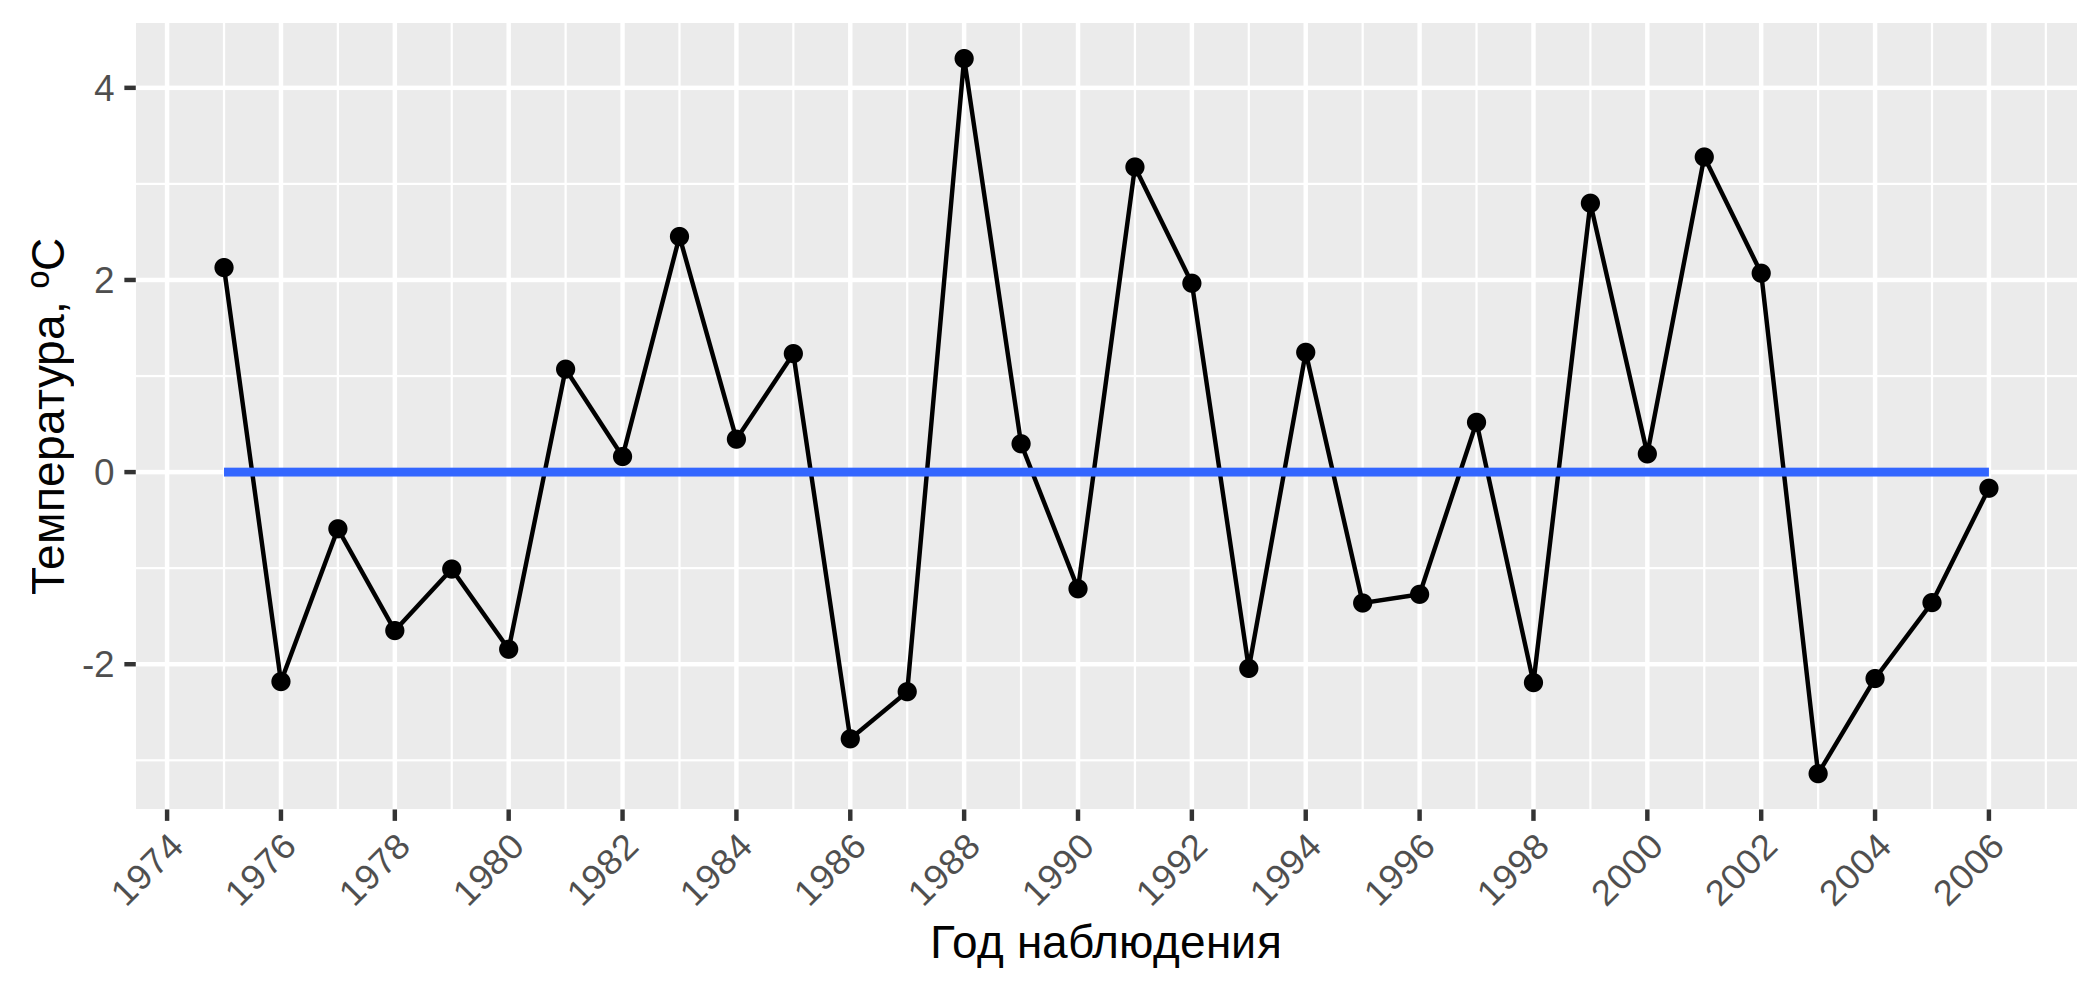
\includegraphics[width=1\linewidth]{../../figures/residual/time-series.png}
    \caption{Ряд остатков $ \varepsilon(t) $}
  \end{figure}
  \end{columns}
\end{frame}

\subsubsection{Качество регрессионной модели}
\begin{frame}
  \frametitle{Качество регрессионной модели}
  \begin{columns}[c]
  \column{3in}
    \begin{itemize}
      \item С помощью критерия Стьюдента, при уровне значимости $ \alpha=0.05 $, доказана значимость коэффициентов регрессионной модели
      \item F-критерий Фишера при уровне значимости $ \alpha = 0.05 $ показал адекватность модели
      \item Точность модели невысока, поскольку коэффициент детерминации $ \eta^2_{x(t)} = 0.275 $
    \end{itemize}
  \column{3in}
    % latex table generated in R 3.1.3 by xtable 1.7-4 package
% Thu May 21 14:09:02 2015
\begin{table}[ht]
\centering
\begin{tabular}{rrrr}
  \hline
 & Год & Актуальное & Прогнозное \\ 
  \hline
1 & 2007 & 19.40 & 18.07 \\ 
  2 & 2008 & 21.80 & 18.18 \\ 
  3 & 2009 & 21.90 & 18.29 \\ 
  4 & 2010 & 24.30 & 18.40 \\ 
  5 & 2011 & 22.80 & 18.51 \\ 
  6 & 2012 & 20.20 & 18.62 \\ 
   \hline
\end{tabular}
\caption{Сравнение прогнозных значений (тренда)} 
\label{table:prediction_trend}
\end{table}

  \end{columns}
\end{frame}

\subsection{Анализ остатков}
\begin{frame}
  \frametitle{Анализ остатков}
  \begin{columns}[c]
  \column{2.5in}
    Визуально и проверкой тестов показана близость выборочного распределения к нормальному \resnormaldistr.

    \vspace{0.5em}

    По графику было сделано предположение об отсутствии значимых автокорреляций. Проведённый тест Льюнга-Бокса подтвердил данное замечание.

    \vspace{0.5em}

    Также было отмечено, что значения имеют небольшую амплитуду и имеют тенденцию к затуханию. Это говорит о стационарности в широком смысле, что показал расширенный тест Дики-Фуллера.
  \column{3.5in}
    \begin{figure}[h]
    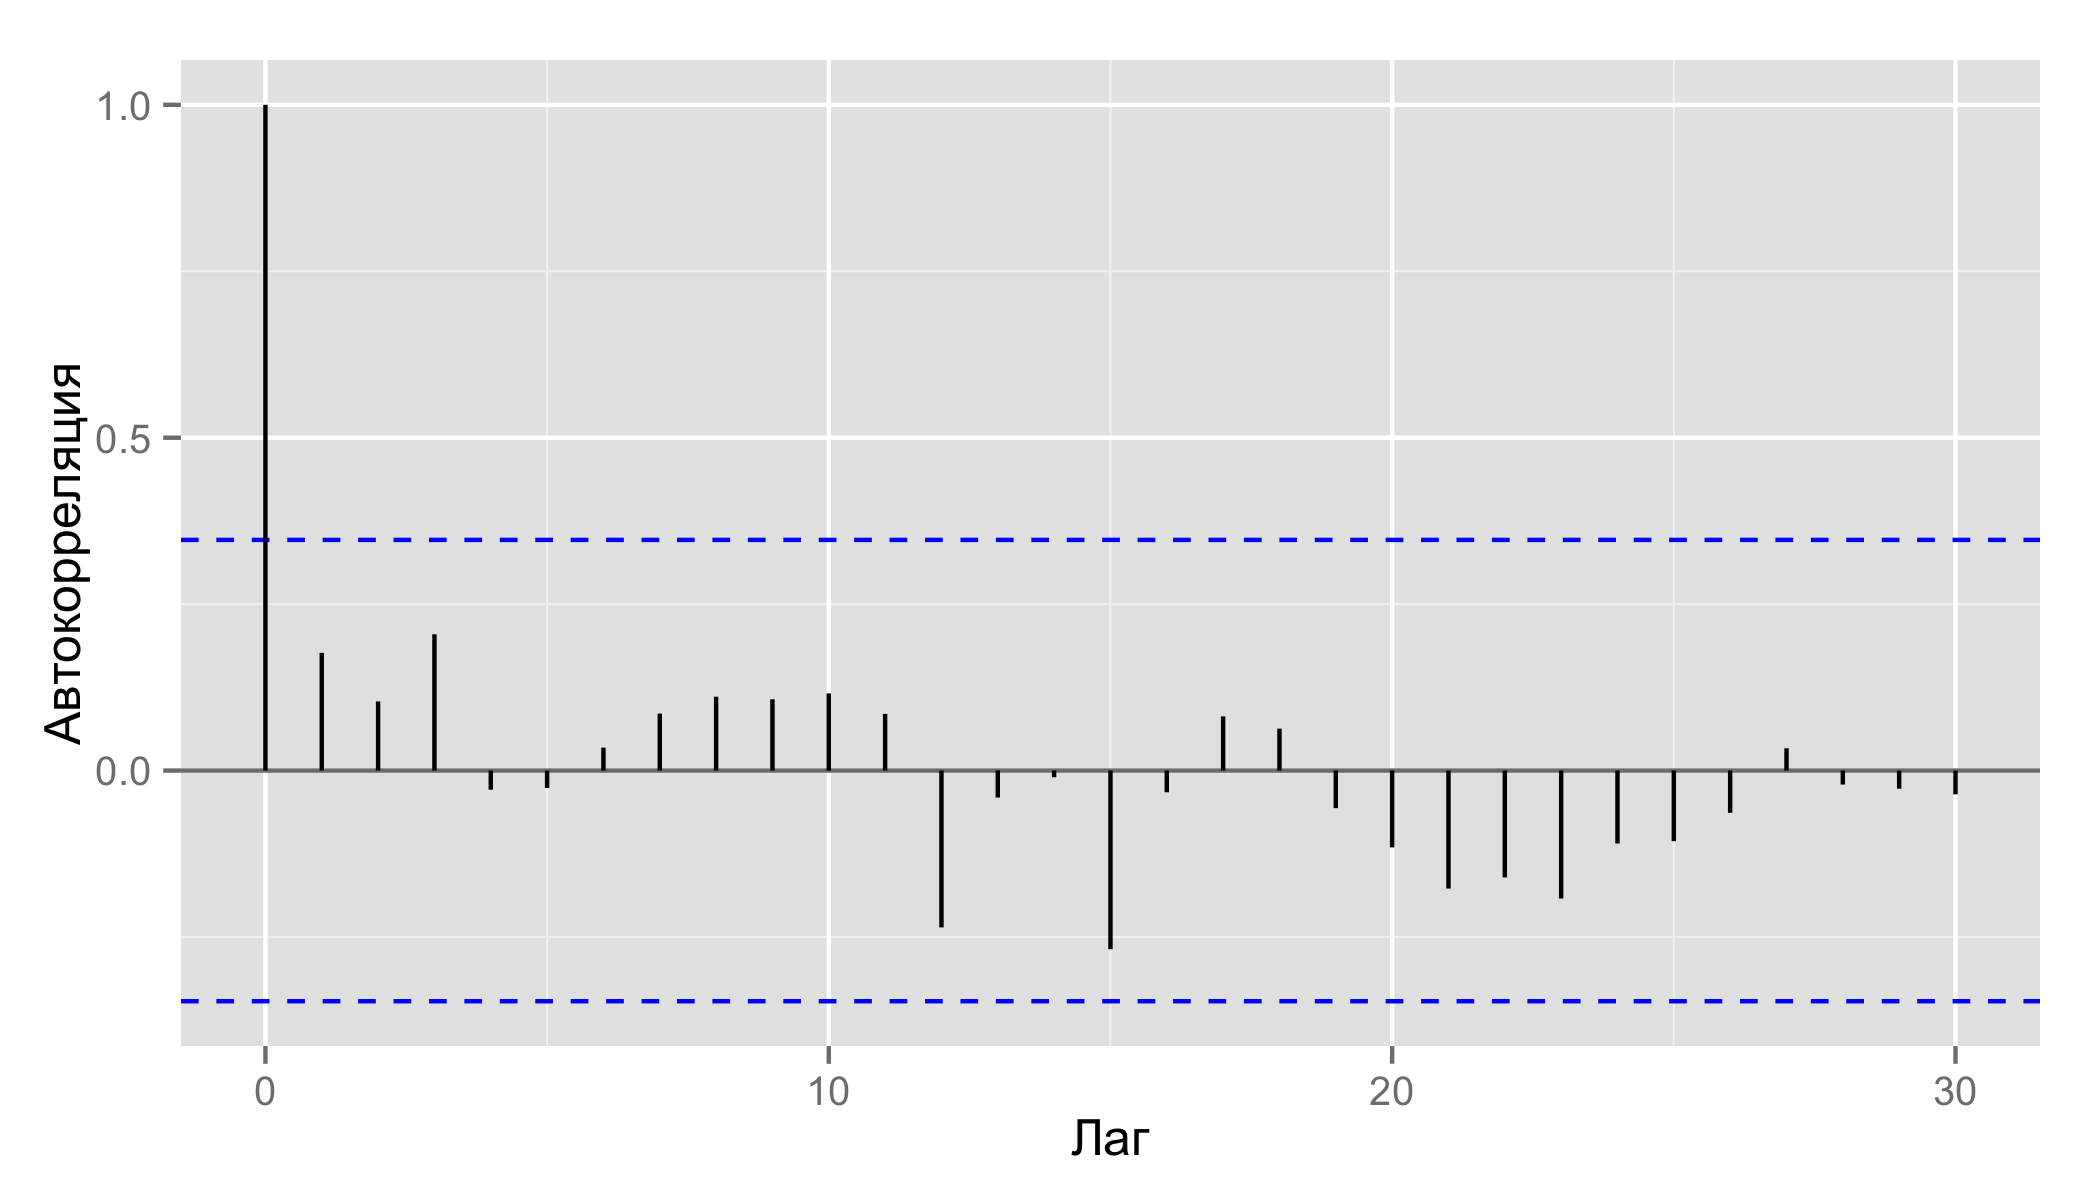
\includegraphics[width=1\linewidth]{../../figures/residual/acf.png}
    \caption{Автокорреляционная функция}
  \end{figure}
  \end{columns}
\end{frame}

\section{Геостатистический подход}

\subsection{Введение}

\begin{frame}
  \frametitle{Оценка вариограммы}
  Рассматривается стационарный в широком смысле гауссовский случайный процесс с дискретным временем $ X(t),~ t \in \mathbb{Z} $, нулевым математическим ожиданием, постоянной дисперсией и неизвестной вариограммой $ 2 \gamma(h), h \in \mathbb{Z} $.
  \begin{Definition}
    \textit{Вариограммой} случайного процесса $ X(t), t \in \mathbb{Z} $, называется функция вида
    \begin{equation}
        2 \gamma (h) = V \{ X(t + h) - X(t) \},~ t, h \in \mathbb{Z}.
    \end{equation}

    При этом функция $ \gamma (h), h \in \mathbb{Z} $, называется \textit{семивариограммой}.
  \end{Definition}
  В качестве оценки вариограммы рассматривается статистика, предложенная Матероном:
  \begin{equation}
    2 \tilde{\gamma}(h) = \frac{1}{n - h} \sum_{t = 1}^{n - h}(X(t + h) - X(t))^2, \quad h = \overline{0, n - 1},
  \end{equation}
\end{frame}

\begin{frame}
  \frametitle{Первые два момента оценки вариограммы}
\begin{Theorem}
  Для оценки $ 2 \tilde{\gamma}(h) $ имеют место следующие соотношения:
  \begin{equation*}
    E \{2 \tilde{\gamma}(h) \} = 2 \gamma(h), % DIRTY HACK
  \end{equation*}
  \begin{equation*}
    cov(2 \tilde{\gamma}(h_1), 2 \tilde{\gamma}(h_2)) =
  \end{equation*}
  \begin{equation*}
    = \frac{2}{(n - h_1)(n - h_2)} \sum_{t = 1}^{n - h_1}\sum_{s = 1}^{n - h_2} (\gamma(t - h_2 - s) + \gamma(t + h_1 - s) - \gamma(t - s) - \gamma(t + h_1 - s - h_2))^2,
  \end{equation*}
  \begin{equation*}
    V \{ 2 \tilde{\gamma}(h) \} = \frac{2}{(n-h)^2}\sum_{t,s = 1}^{n - h} ( \gamma(t - h - s) + \gamma(t + h - s) - 2\gamma(t - s) )^2,
  \end{equation*}
  где $ \gamma(h), h \in \mathbb{Z} $, --- семивариограмма процесса $ X(t), t \in \mathbb{Z}$, $ h, h_1, h_2 = \overline{0, n - 1} $.
\end{Theorem}
\end{frame}

\begin{frame}
  \frametitle{Асимптотическое поведение оценки вариограммы}
  \begin{Theorem}
  Если имеет место соотношение
  \begin{equation*}
    \sum_{h = -\infty}^{+\infty} \vert \gamma(h) \vert < +\infty, \text{то}
  \end{equation*}
  \begin{equation*}
    \lim_{n \to \infty} (n - \min\{ h_1, h_2 \}) cov\{ 2 \tilde{\gamma}(h_1), 2 \tilde{\gamma}(h_2) \} = 2 \sum_{m = -\infty}^{+\infty} \gamma(m - h_2) + \gamma(m + h_1) - \gamma(m) - \gamma(m + h_1 - h_2))^2,
  \end{equation*}
  \begin{equation*}
    \lim_{n \to \infty} (n - h) V\{ 2 \tilde{\gamma}(h) \} = 2 \sum_{m = -\infty}^{+\infty} \gamma(m - h) + \gamma(m + h) - 2 \gamma(m))^2.
  \end{equation*}
  где $ \gamma(h), h \in \mathbb{Z} $, --- семивариограмма процесса $ X(t), t \in \mathbb{Z}$, $ h, h_1, h_2 = \overline{0, n - 1} $.
\end{Theorem}
\end{frame}

\subsection{Вариограммный анализ}

\begin{frame}
  \frametitle{График экспериментальной вариограммы}
   \begin{columns}[c]
   \column{4.5in}
  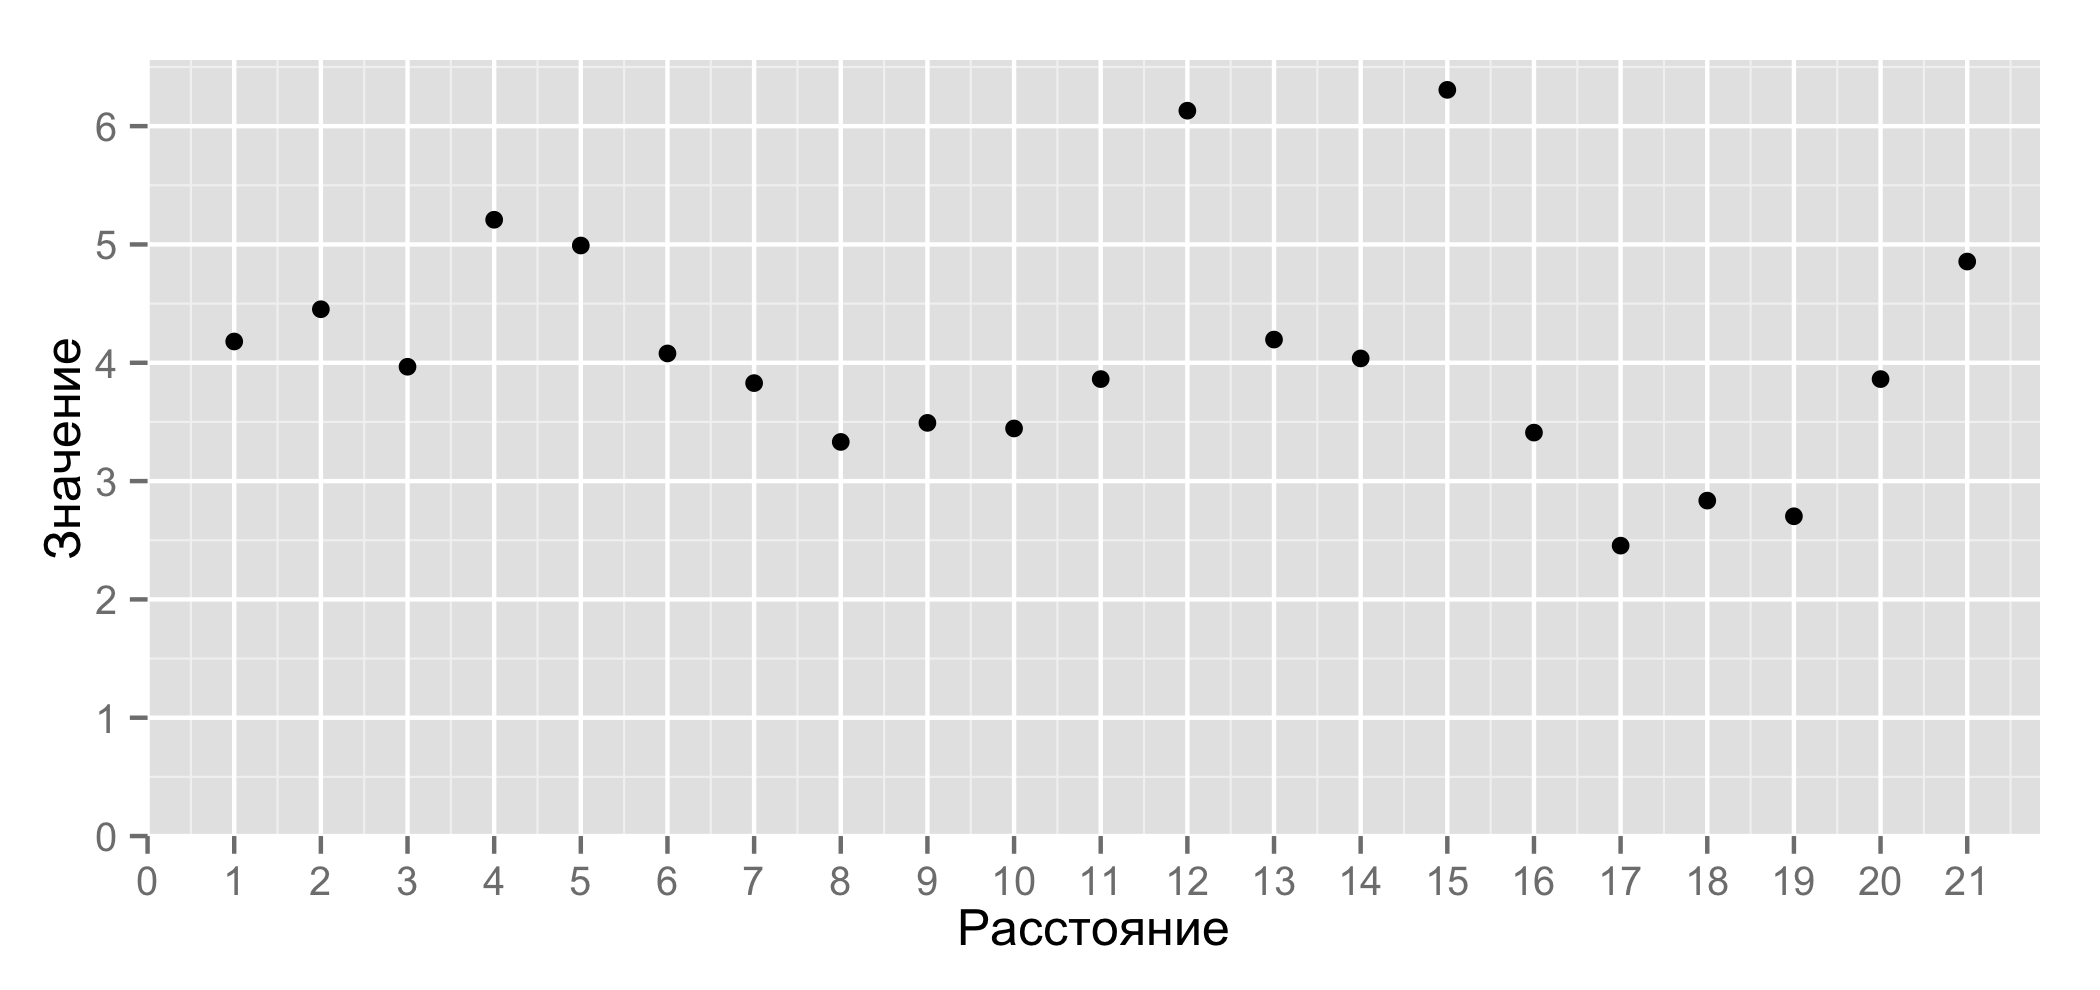
\includegraphics[width=0.95\textwidth]{../../figures/variogram/lin-variogram.png}
  \end{columns}
\end{frame}

\begin{frame}
  \frametitle{Линейная модель}
  \begin{columns}[c]
  \column{3in}
  \begin{equation}\begin{gathered}
  \label{eq:lin}
    \widehat{\gamma}(h) = c_0 + Lin(h) = \left\{
   \begin{array}{l l}
     c_0 + b \cdot h, & h > 0, \\
     c_0, & h \leq 0,
   \end{array} \right.
  \end{gathered}\end{equation}
  где $ b $ -- параметр, отвечающий за угол наклона, $ c_0 $ --- эффект самородков.

  \vspace{0.5em}

  Подобранная модель:
  \begin{equation}
  \label{eq:gamma1}
    \widehat{\gamma}_1(h) = Lin(h), \quad b = 4,
  \end{equation}

  Показатели качества
  \begin{equation*}
    r_{\varepsilon\varepsilon^{*}} = -0.09129, \quad MSE = 6.324
  \end{equation*}

  \column{3in}
  \vspace{-14.5pt}
  \begin{figure}[H]
    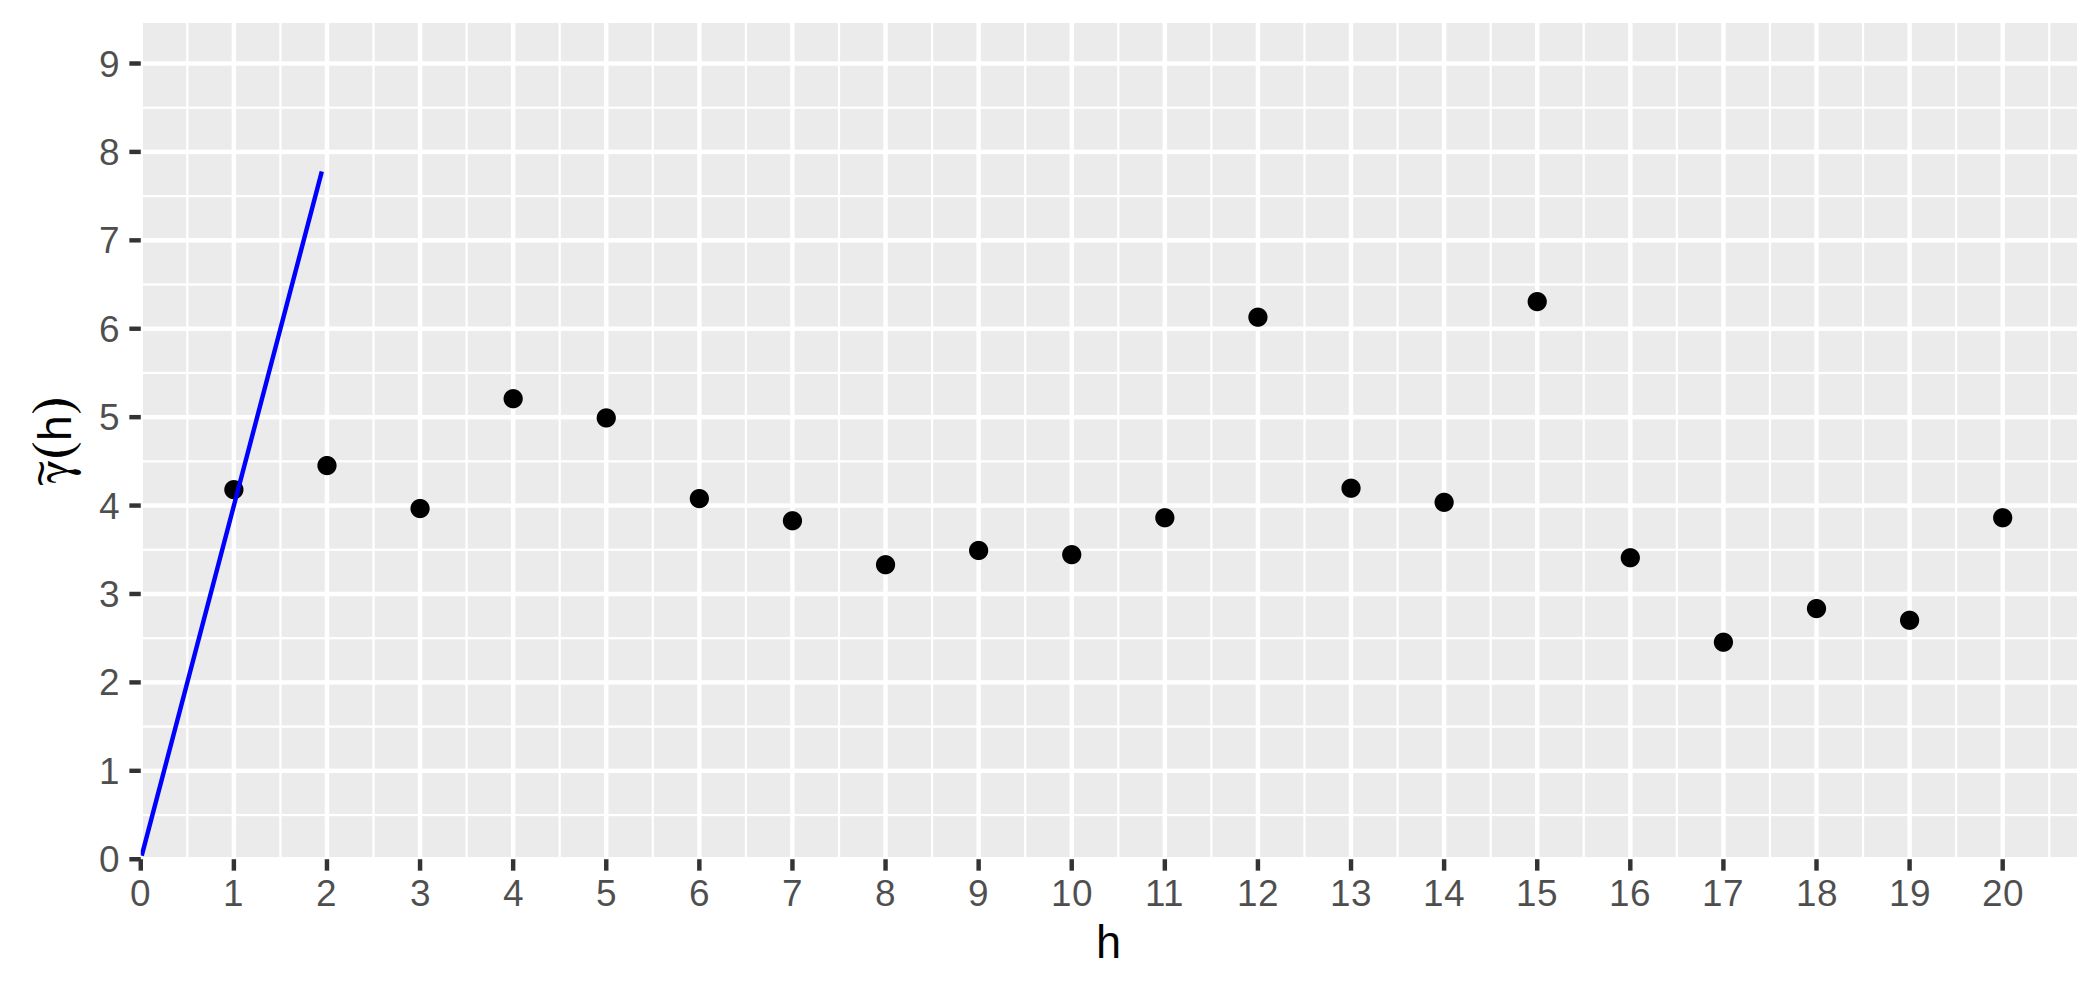
\includegraphics[width=0.9\linewidth]{../../figures/variogram/lin-modeled.png} \\
    \caption{Модель семивариограммы $\widehat{\gamma}_1(h)$}
    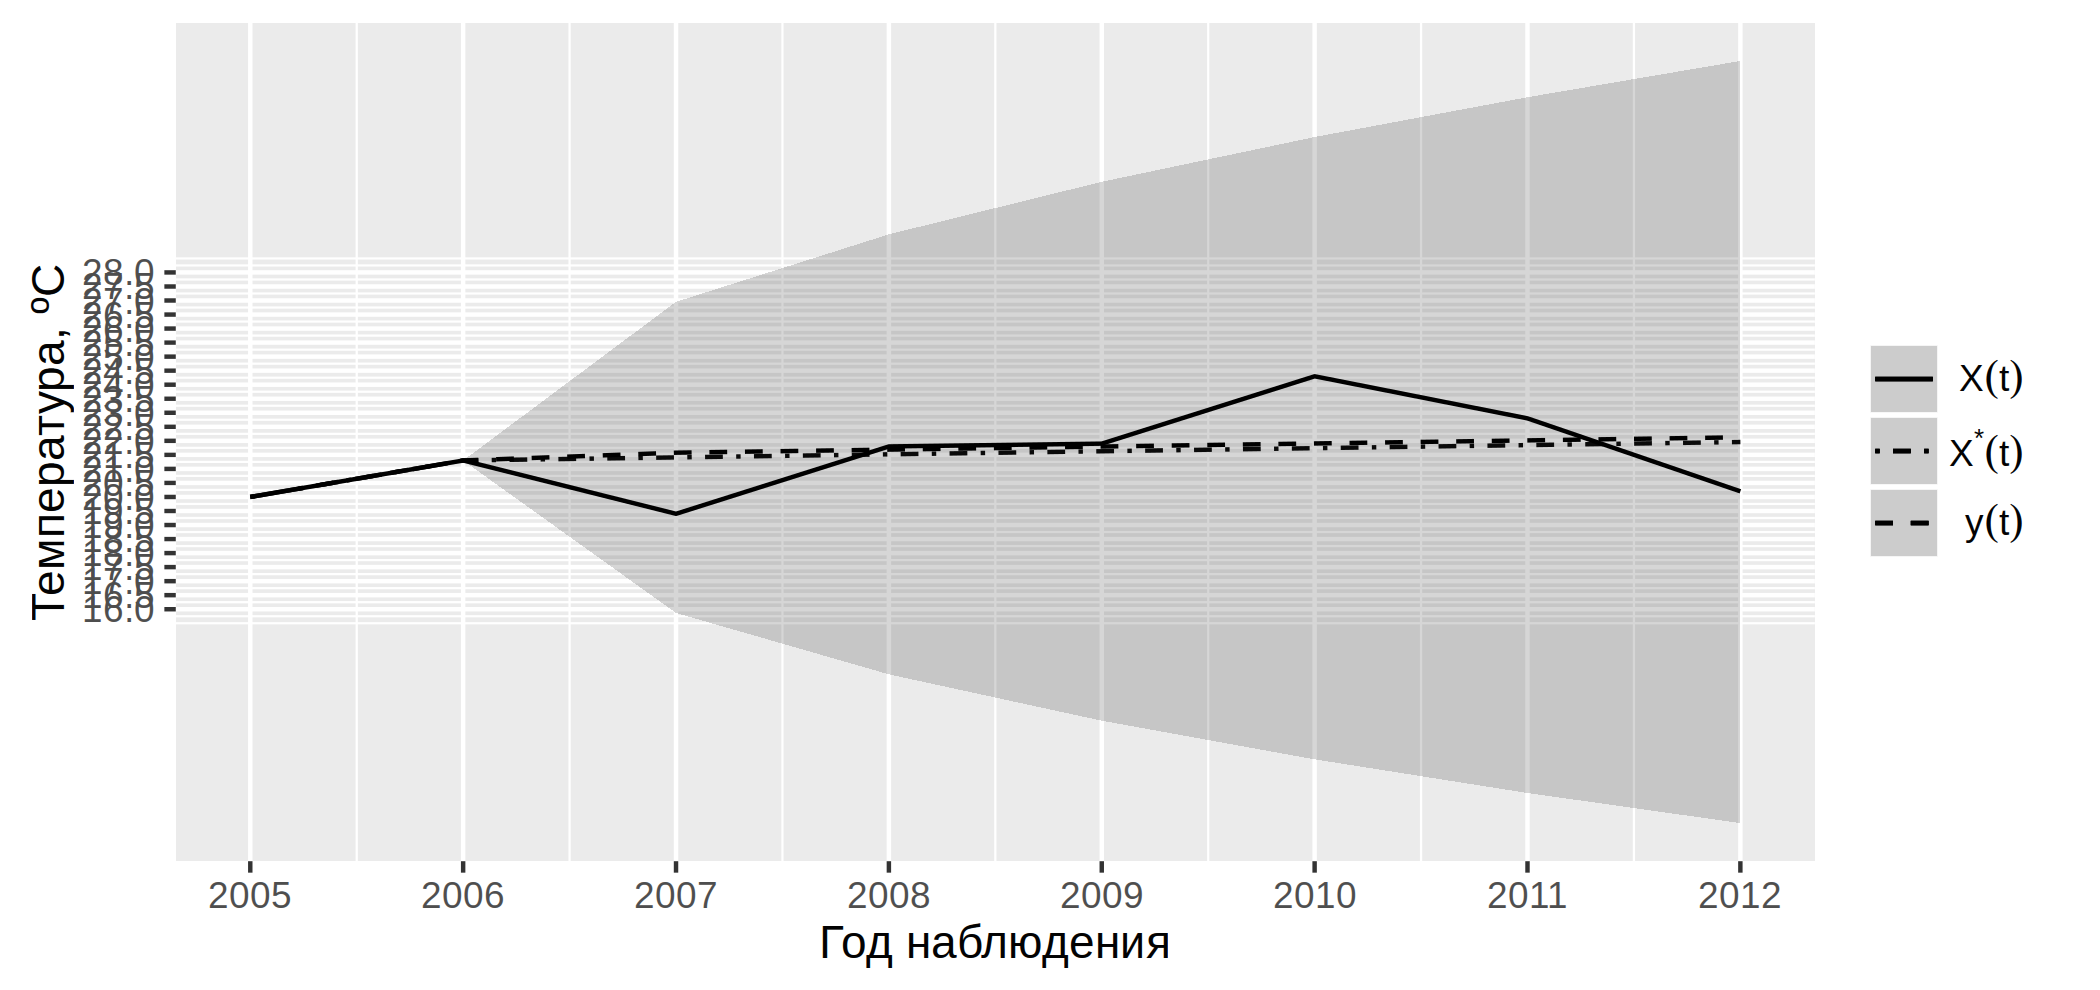
\includegraphics[width=0.9\linewidth]{../../figures/variogram/lin-cross-prediction.png}
    \caption{Прогноз по модели $\widehat{\gamma}_1(h)$}
  \end{figure}
  \end{columns}
\end{frame}

\begin{frame}
  \frametitle{Чистый эффект самородков}
  \begin{columns}[c]
  \column{3in}
  \begin{equation}\begin{gathered}
  \label{eq:nug}
    \widehat{\gamma}(h) = c \cdot Nug(h) = \left\{
   \begin{array}{l l}
     0, & h = 0, \\
     c, & h \neq 0,
   \end{array} \right.
  \end{gathered}\end{equation}
  где $ b $ -- параметр, отвечающий за угол наклона, $ c_0 $ --- эффект самородков.

  \vspace{0.5em}

  Подобранная модель:
  \begin{equation}
  \label{eq:gamma2}
    \widehat{\gamma}_2(h) = 4.04 \cdot Nug(h).
  \end{equation}

  Показатели качества
  \begin{equation*}
    r_{\varepsilon\varepsilon^{*}} = -1, \quad MSE = 4.199
  \end{equation*}

  \column{3in}
  \vspace{-14.5pt}
  \begin{figure}[H]
    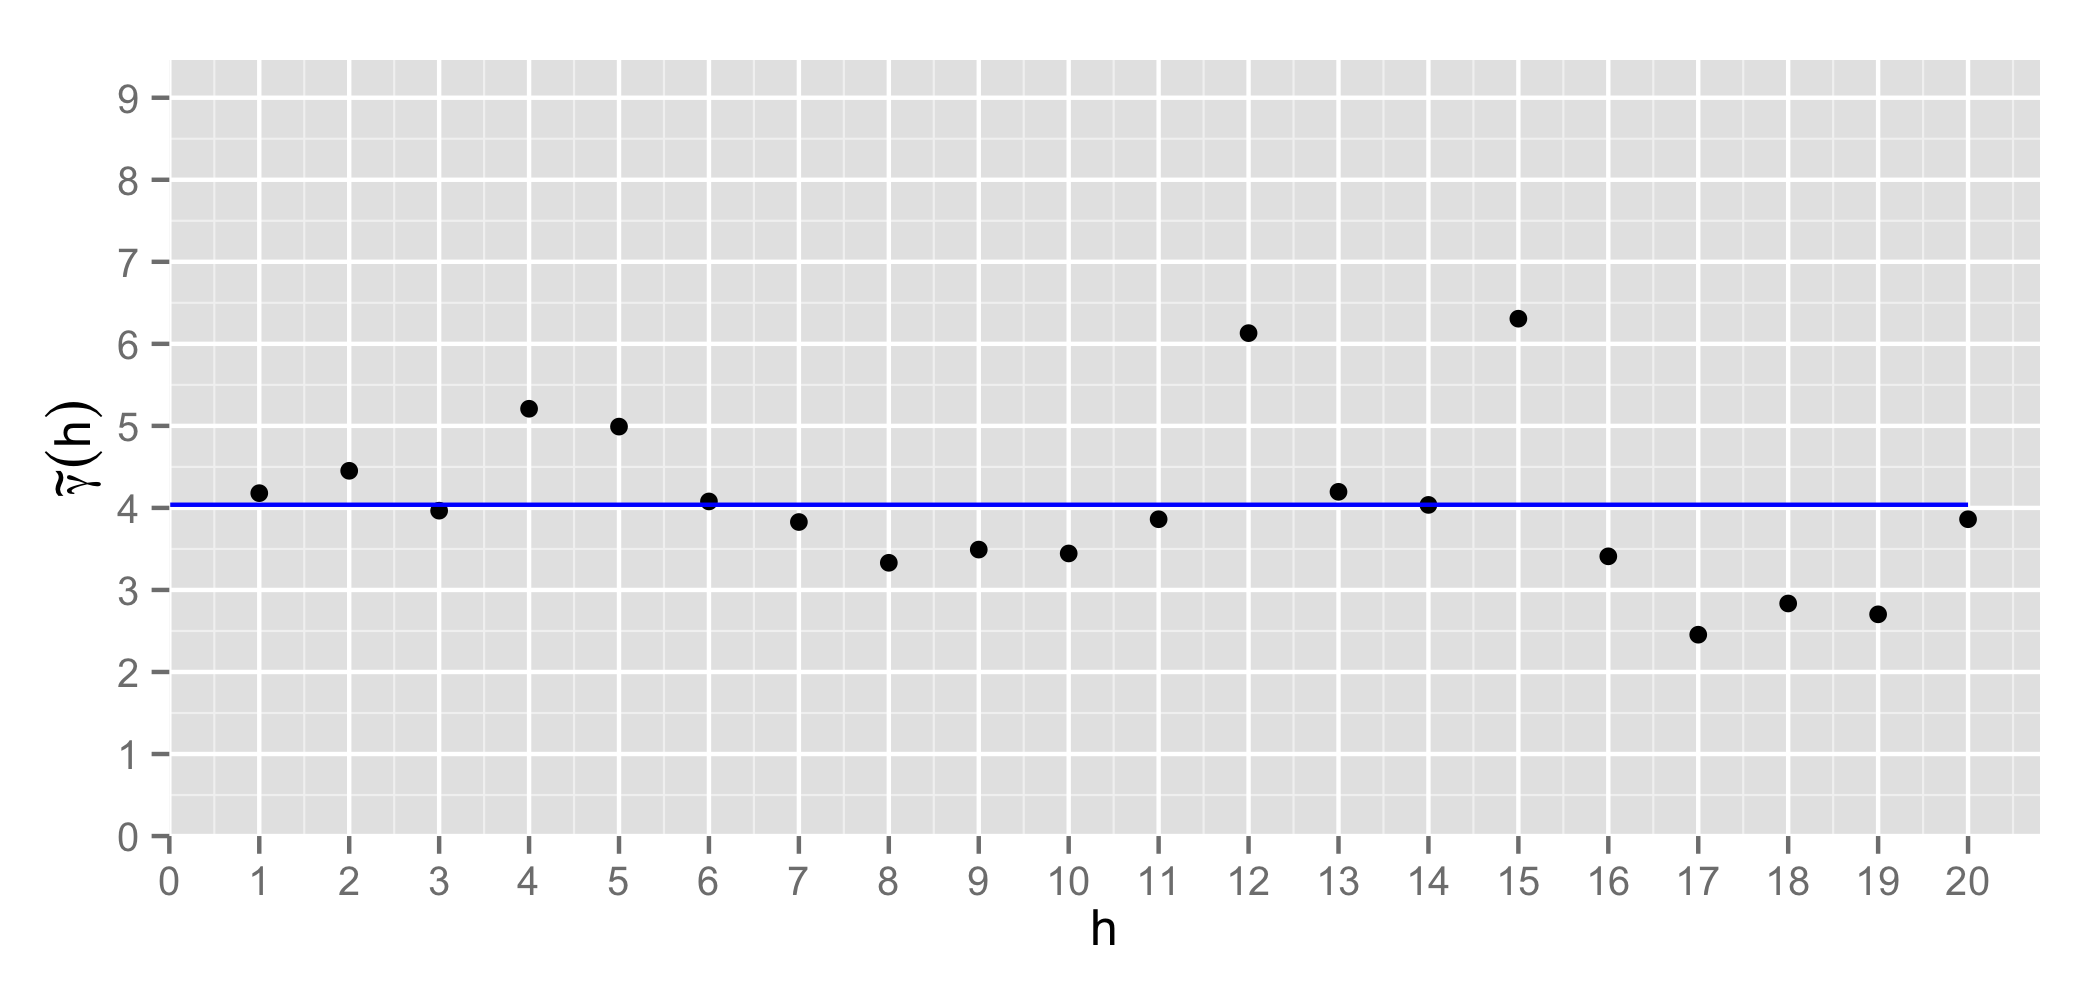
\includegraphics[width=0.9\linewidth]{../../figures/variogram/lin-fit-modeled.png} \\
    \caption{Модель семивариограммы $\widehat{\gamma}_1(h)$}
    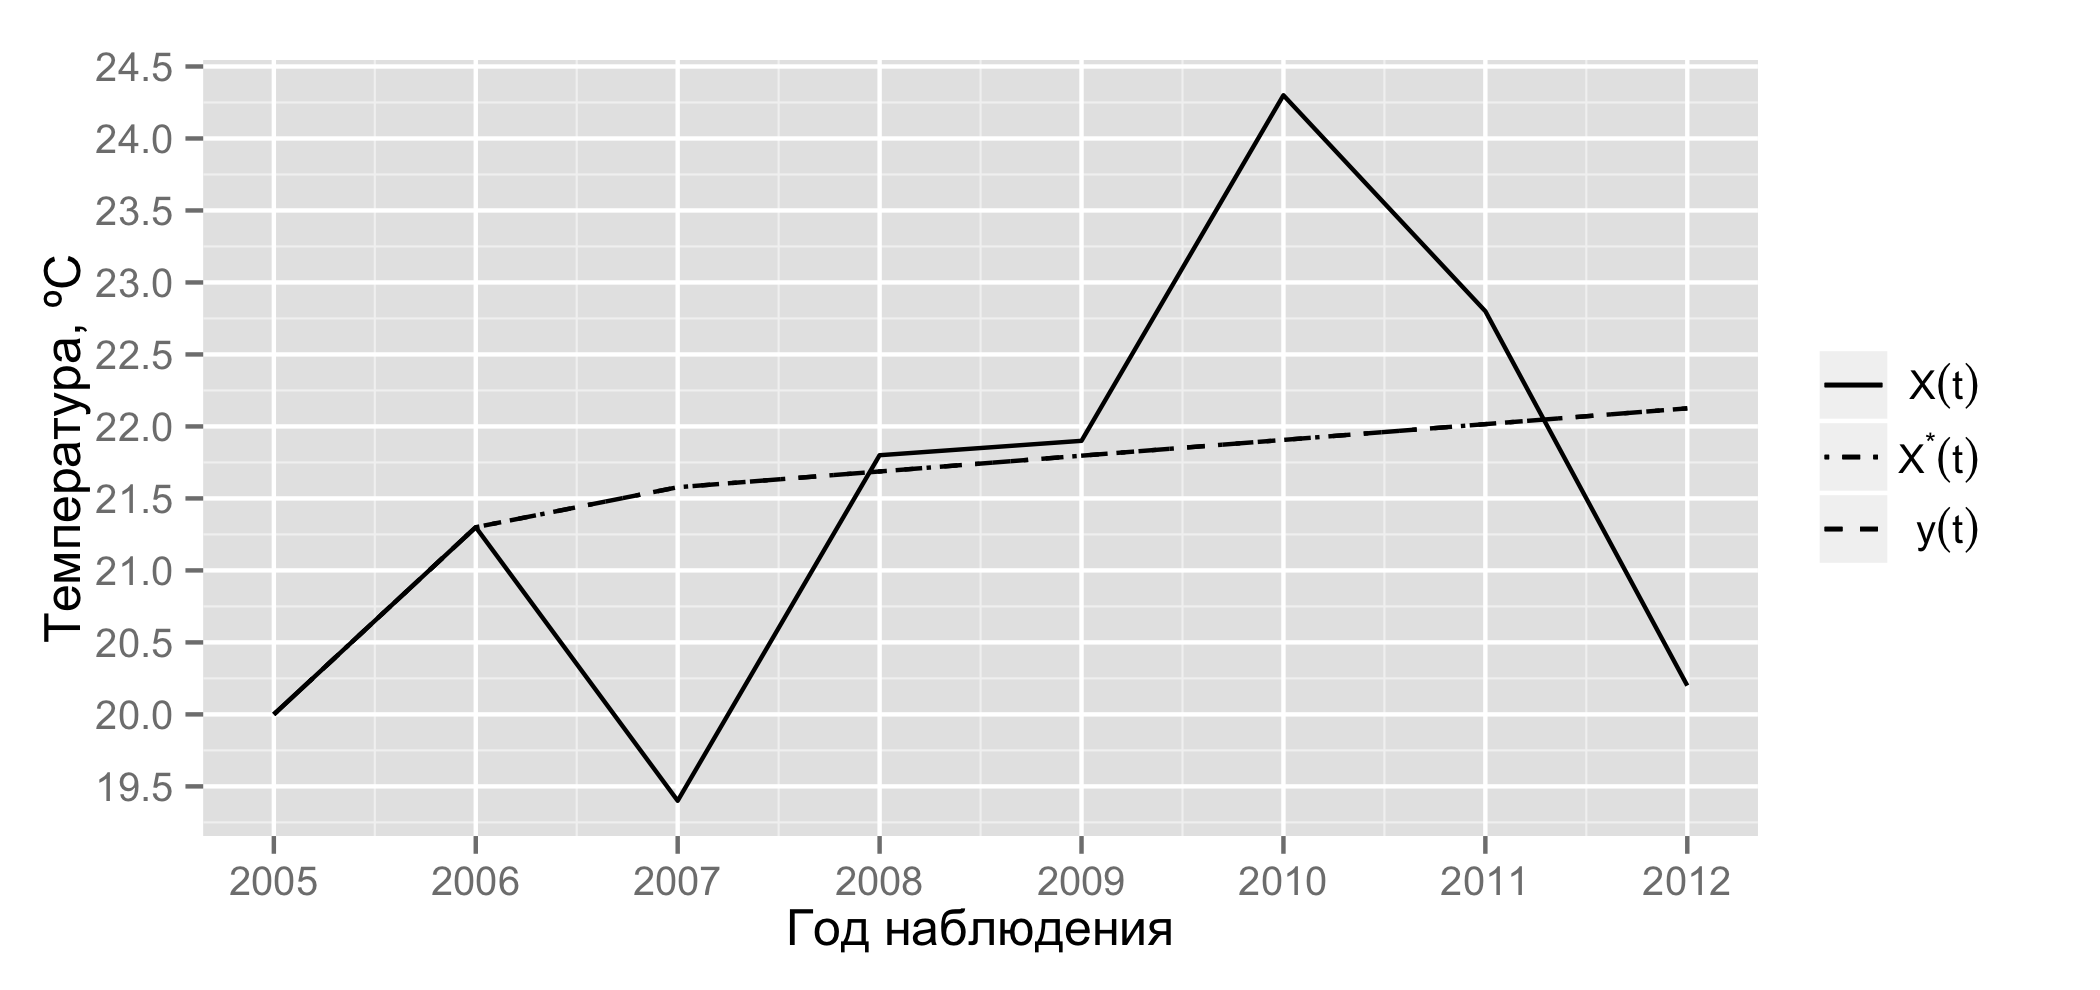
\includegraphics[width=0.9\linewidth]{../../figures/variogram/lin-fit-cross-prediction.png}
    \caption{Прогноз по модели $\widehat{\gamma}_1(h)$}
  \end{figure}
  \end{columns}
\end{frame}

\begin{frame}
  \frametitle{Линейная модель с порогом}
  \begin{columns}[c]
  \column{3in}
  \begin{equation}\begin{gathered}
  \label{eq:linsill}
    \widehat{\gamma}(h) = c_0 + c \cdot Lin(h, a) = \\
    = \left\{
    \begin{array}{l l}
     c_0 + c \cdot \frac{h}{a}, & 0 \leq h \leq a, \\
     c_0 + c, & h > a,
    \end{array} \right.
  \end{gathered}\end{equation}
  где $ c_0 $ -- эффект самородков, $ c $ -- порог, $ a $ -- ранг.

  \vspace{0.5em}

  Подобранная модель:
  \begin{equation}
  \label{eq:gamma4}
    \widehat{\gamma}_4(h) = 4 \cdot Lin(h, 2).
  \end{equation}

  Показатели качества
  \begin{equation*}
    r_{\varepsilon\varepsilon^{*}} = 0.152, \quad MSE = 18.69
  \end{equation*}

  \column{3in}
  \vspace{-14.5pt}
  \begin{figure}[H]
    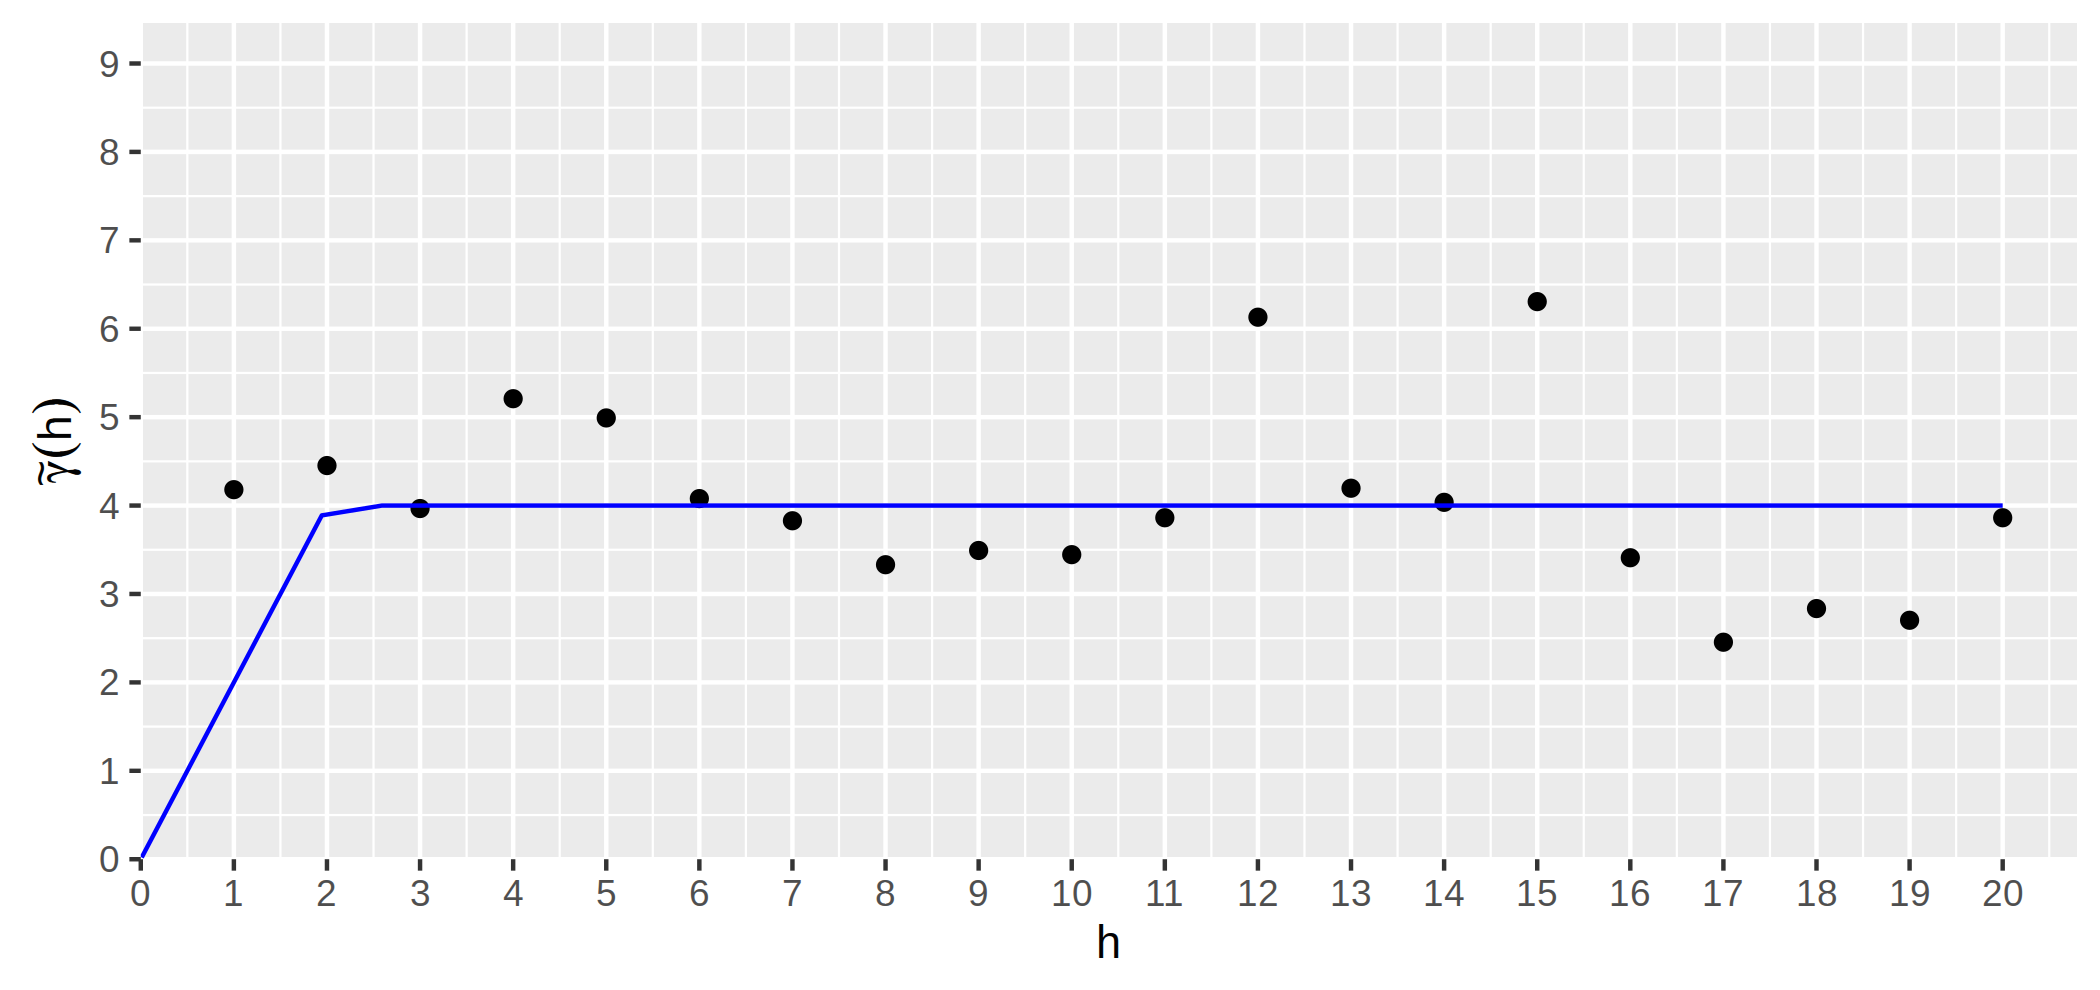
\includegraphics[width=0.9\linewidth]{../../figures/variogram/lin-fit-adapt-modeled.png} \\
    \caption{Модель семивариограммы $\widehat{\gamma}_4(h)$}
    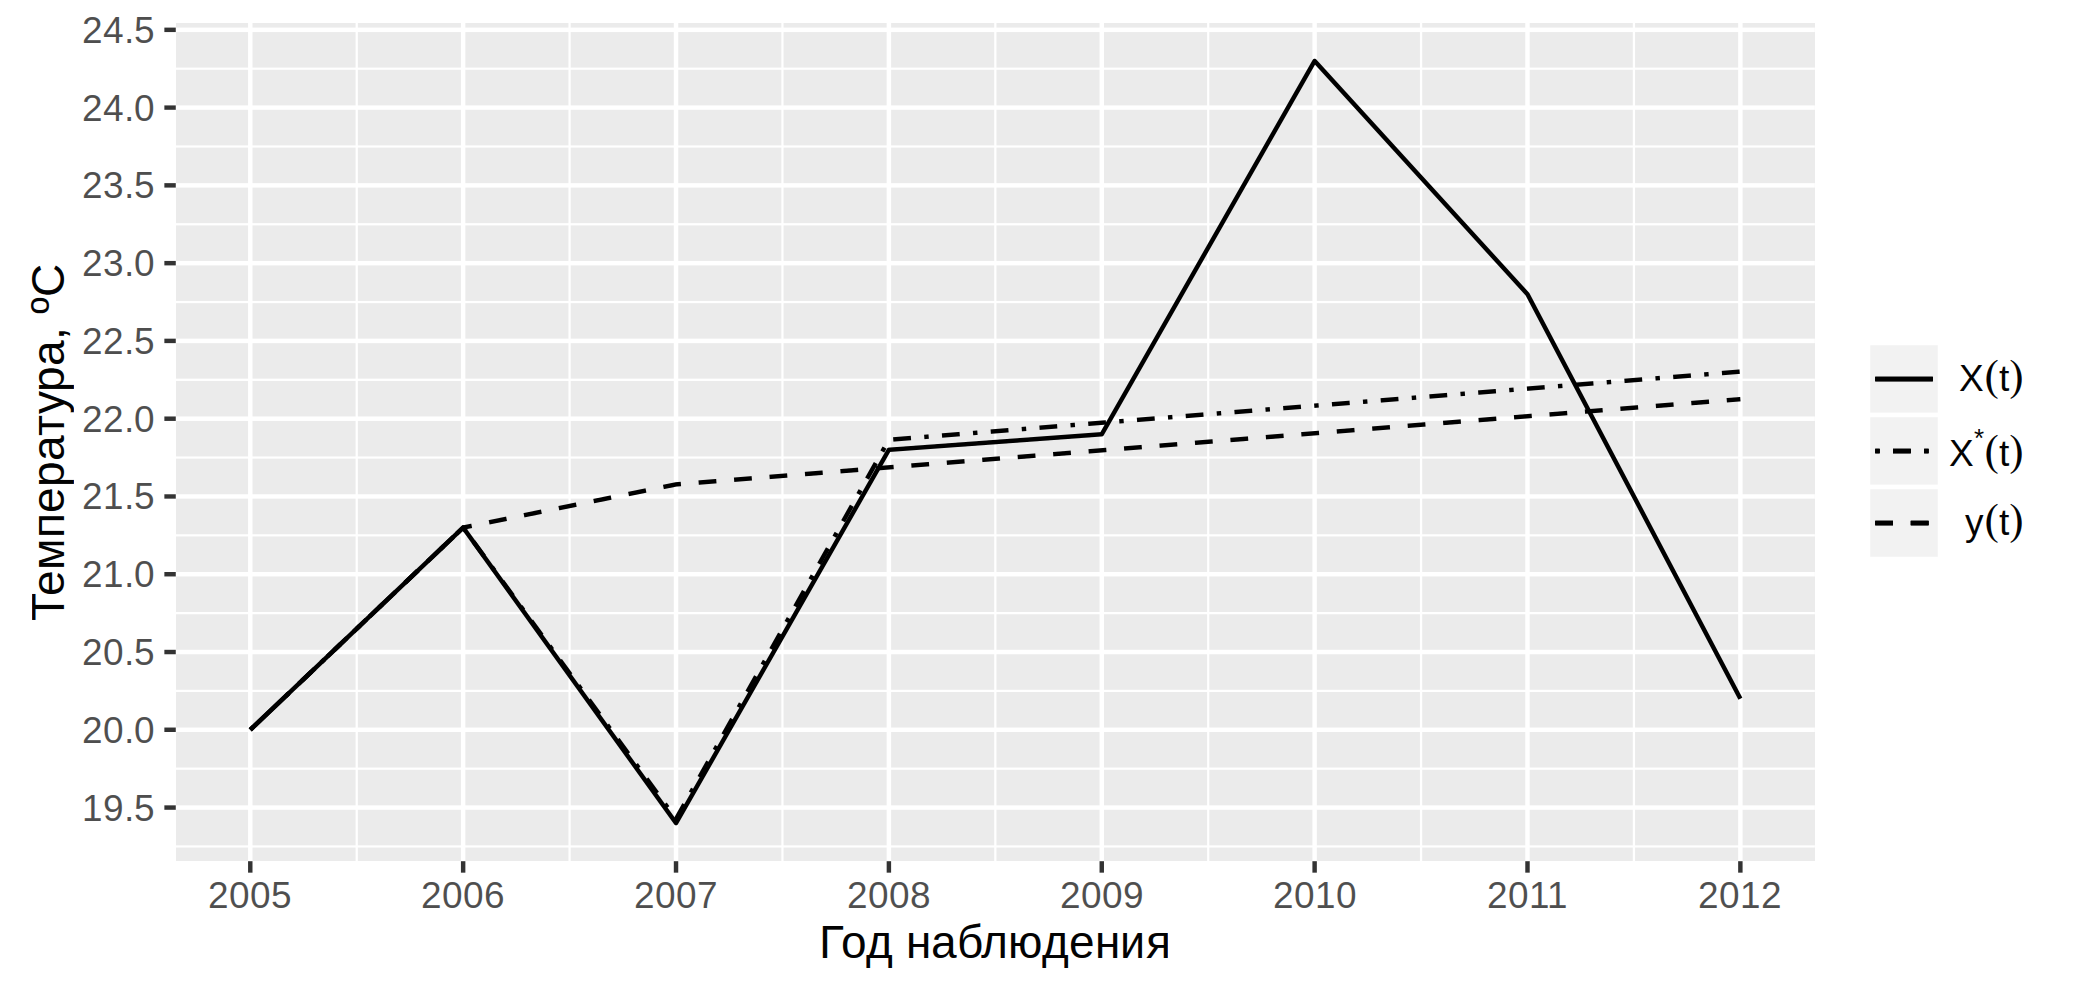
\includegraphics[width=0.9\linewidth]{../../figures/variogram/lin-fit-adapt-cross-prediction.png}
    \caption{Прогноз по модели $\widehat{\gamma}_4(h)$}
  \end{figure}
  \end{columns}
\end{frame}

\begin{frame}
  \frametitle{Сферическая модель}
  \begin{columns}[c]
  \column{3in}
  \begin{equation}\begin{gathered}
  \label{eq:sph}
    \widehat{\gamma}(h) = c_0 + c \cdot Sph(h, a) = \\
    = \left\{
    \begin{array}{l l}
      c_0 + c \cdot (\frac{3}{2} \frac{h}{a} - \frac{1}{2}(\frac{h}{a})^3), & h \le a, \\
      c_0 + c, & h \geq a,
    \end{array} \right.
  \end{gathered}\end{equation}
  где $ c_0 $ -- эффект самородков, $ c $ -- порог, $ a $ -- ранг.

  \vspace{0.5em}

  Подобранная модель:
  \begin{equation}
  \label{eq:gamma5}
    \widehat{\gamma}_5(h) = 0.9 + 4 Sph(h, 6.9),
  \end{equation}

  Показатели качества
  \begin{equation*}
    r_{\varepsilon\varepsilon^{*}} = -0.009, \quad MSE = 5.396
  \end{equation*}

  \column{3in}
  \vspace{-14.5pt}
  \begin{figure}[H]
    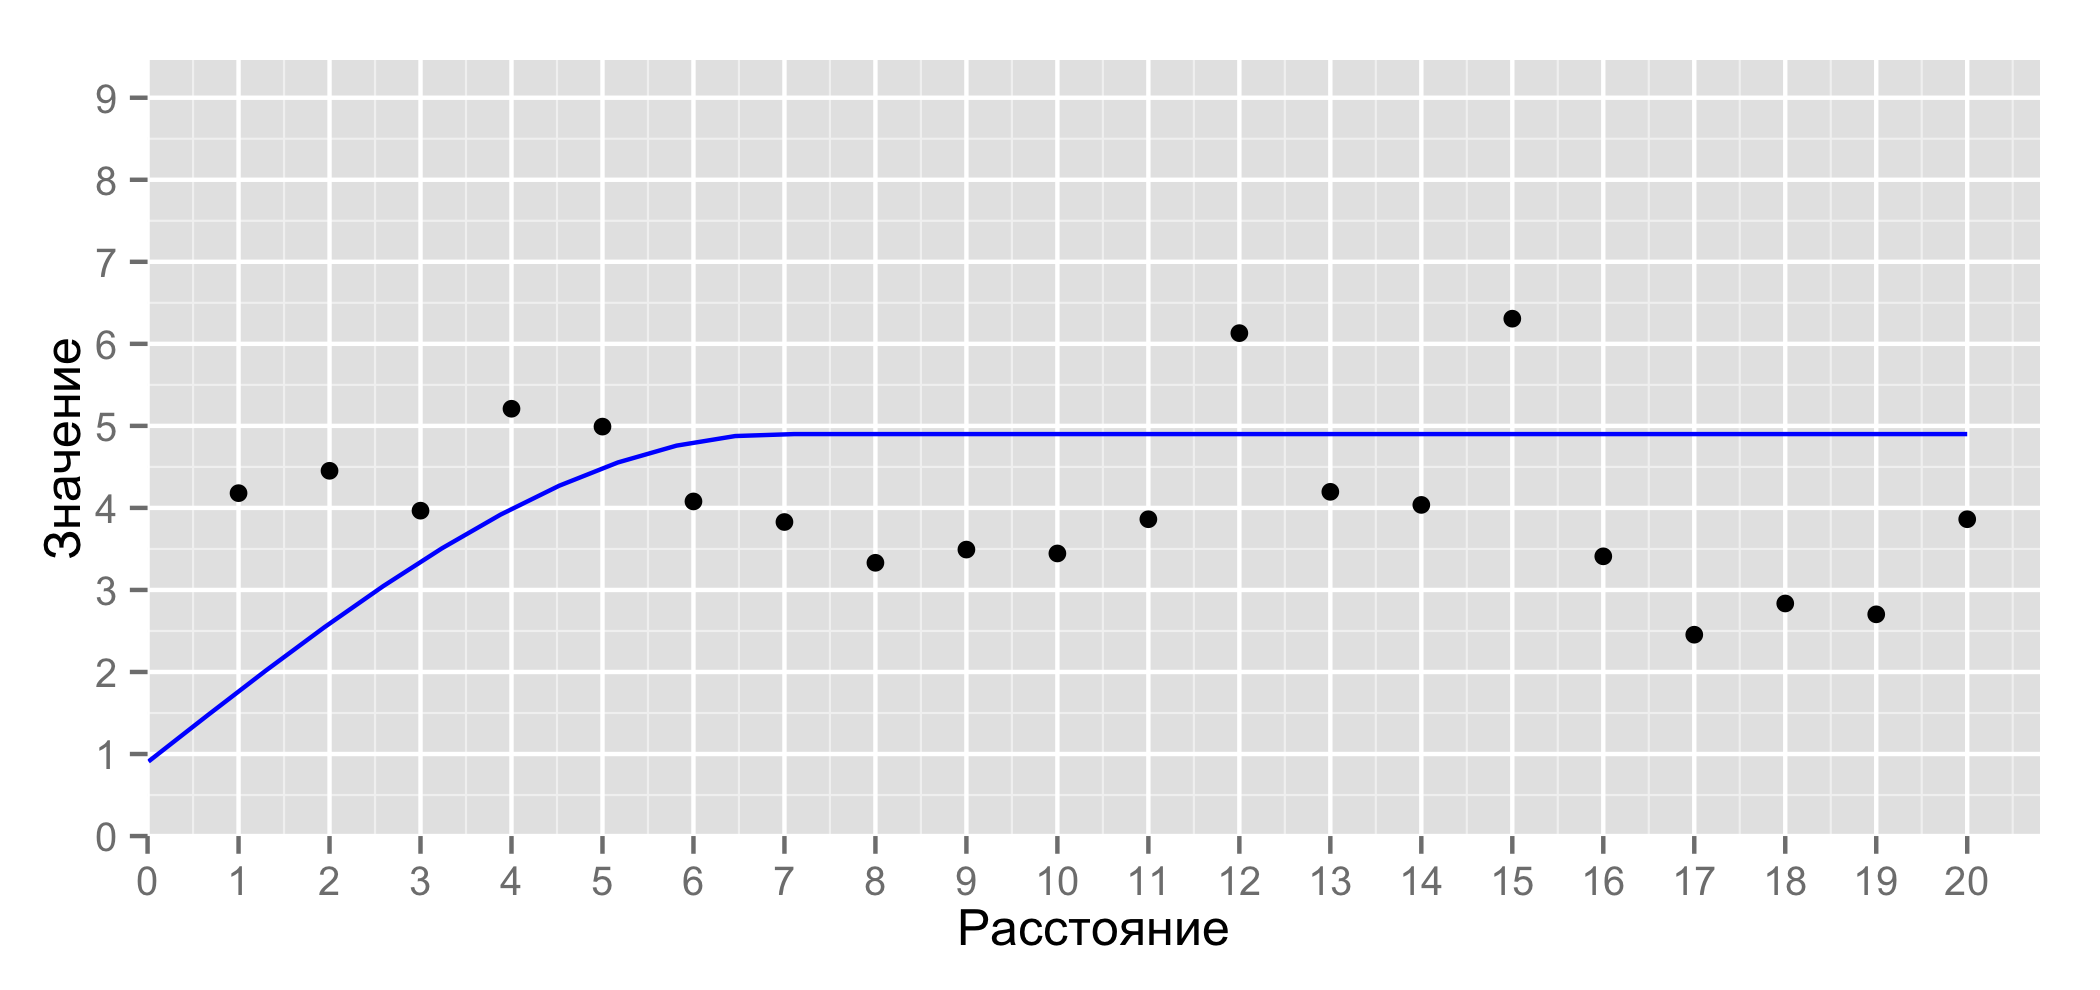
\includegraphics[width=0.9\linewidth]{../../figures/variogram/sph-fit-adapt-modeled.png} \\
    \caption{Модель семивариограммы $\widehat{\gamma}_5(h)$}
    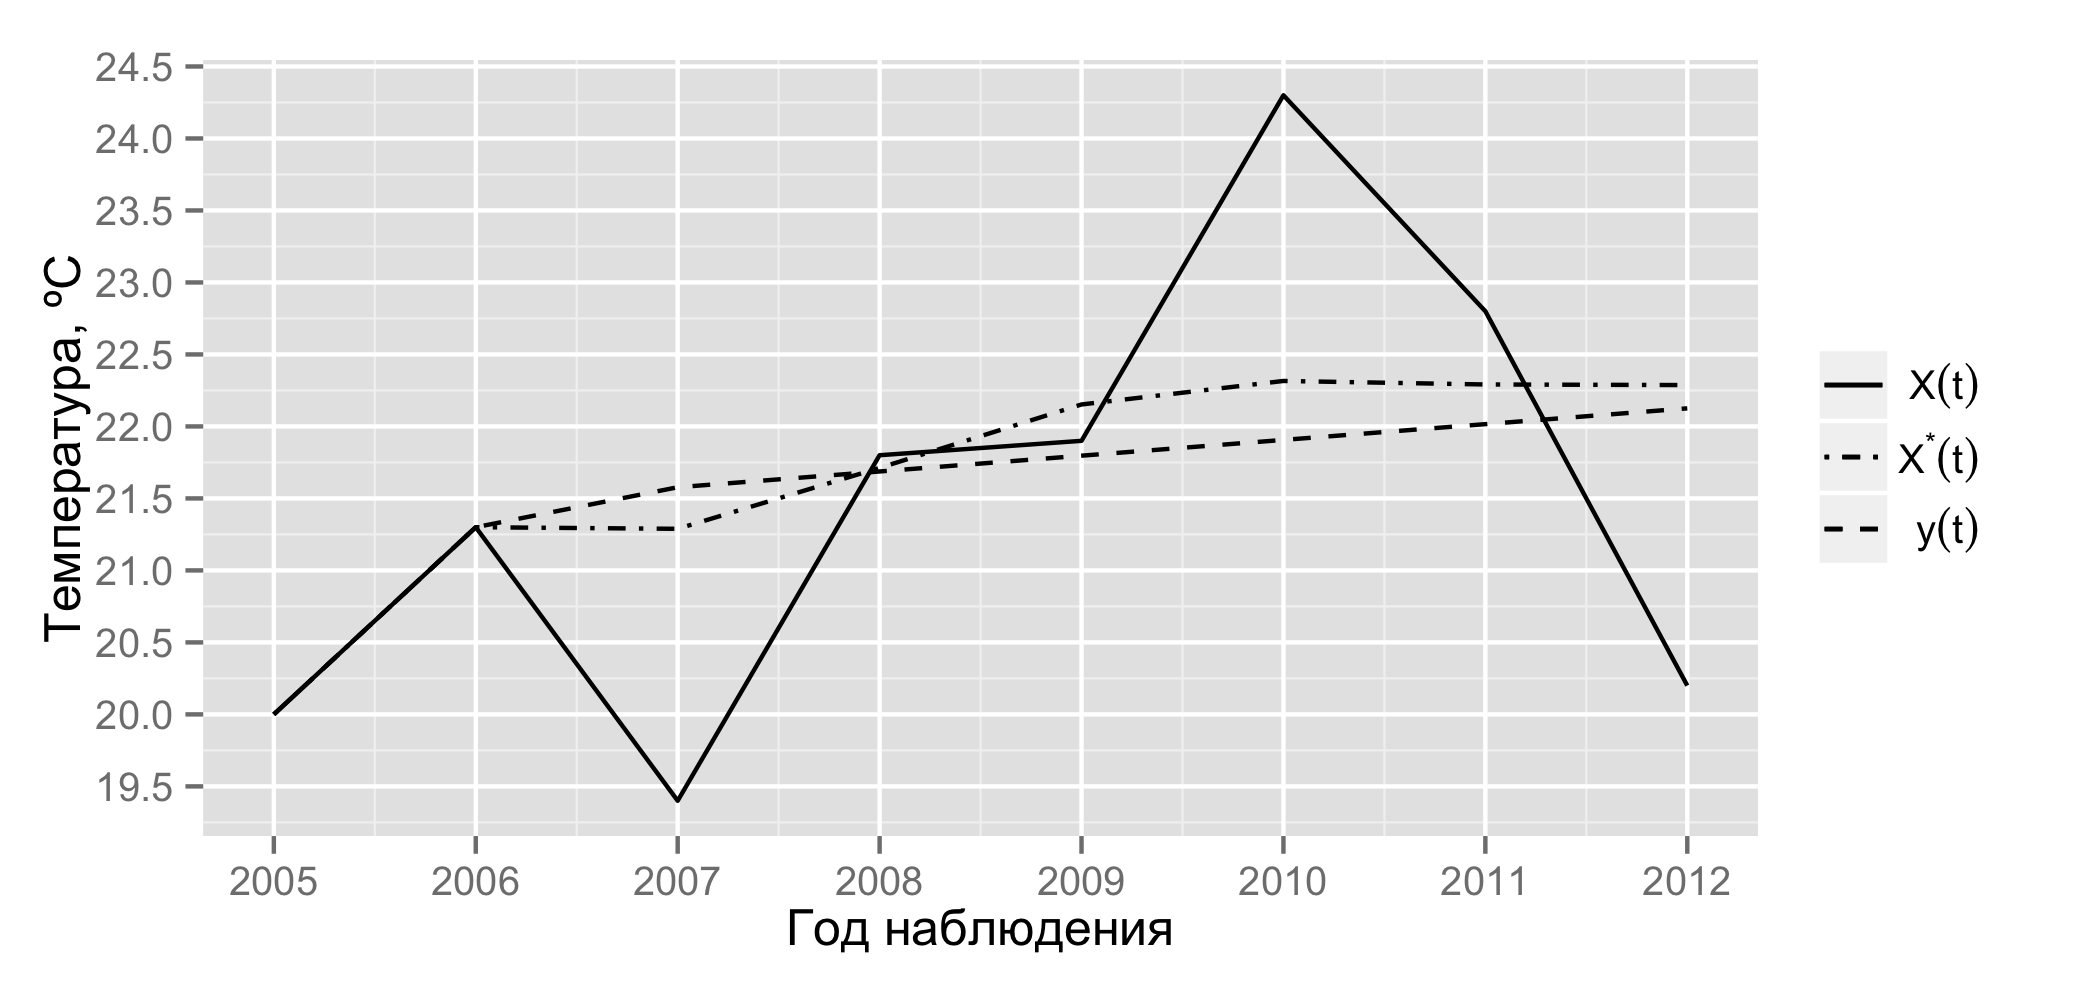
\includegraphics[width=0.9\linewidth]{../../figures/variogram/sph-fit-adapt-cross-prediction.png}
    \caption{Прогноз по модели $\widehat{\gamma}_5(h)$}
  \end{figure}
  \end{columns}
\end{frame}

\begin{frame}
  \frametitle{Периодическая модель}
  \begin{columns}[c]
  \column{3in}
  \begin{equation}
  \label{eq:per}
    \widehat{\gamma}(h) = c_0 + c \cdot Per(h, a) = 1 - cos(\frac{2 \pi h}{a}),
  \end{equation}
  где $ c_0 $ -- эффект самородков, $ c $ -- порог, $ a $ -- ранг.

  \vspace{0.5em}

  Подобранная модель:
  \begin{equation}
  \label{eq:gamma6}
    \widehat{\gamma}_6(h) = 4 \cdot Per(h, 0.898),
  \end{equation}

  Показатели качества
  \begin{equation*}
    r_{\varepsilon\varepsilon^{*}} = 0.404, \quad MSE = 4.369
  \end{equation*}

  \column{3in}
  \vspace{-14.5pt}
  \begin{figure}[H]
    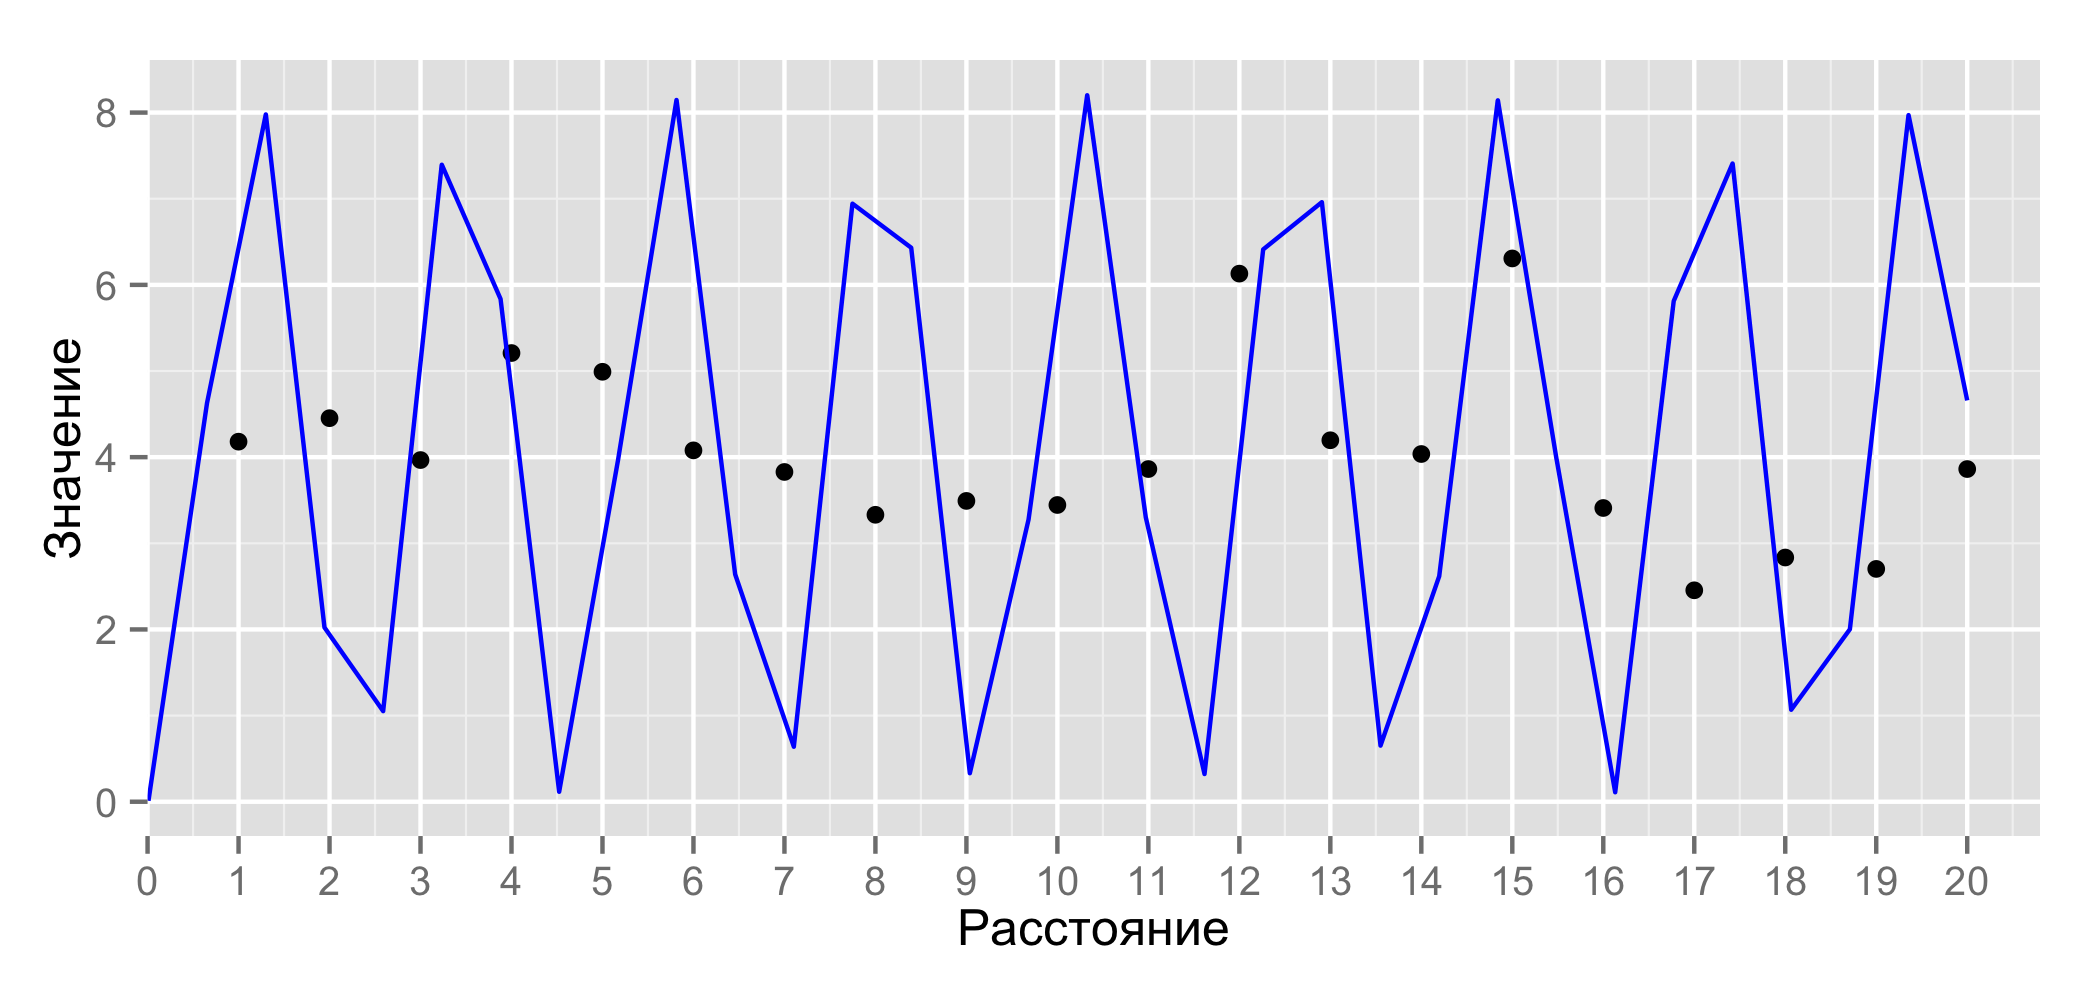
\includegraphics[width=0.9\linewidth]{../../figures/variogram/per-fit-cv-modeled.png} \\
    \caption{Модель семивариограммы $\widehat{\gamma}_6(h)$}
    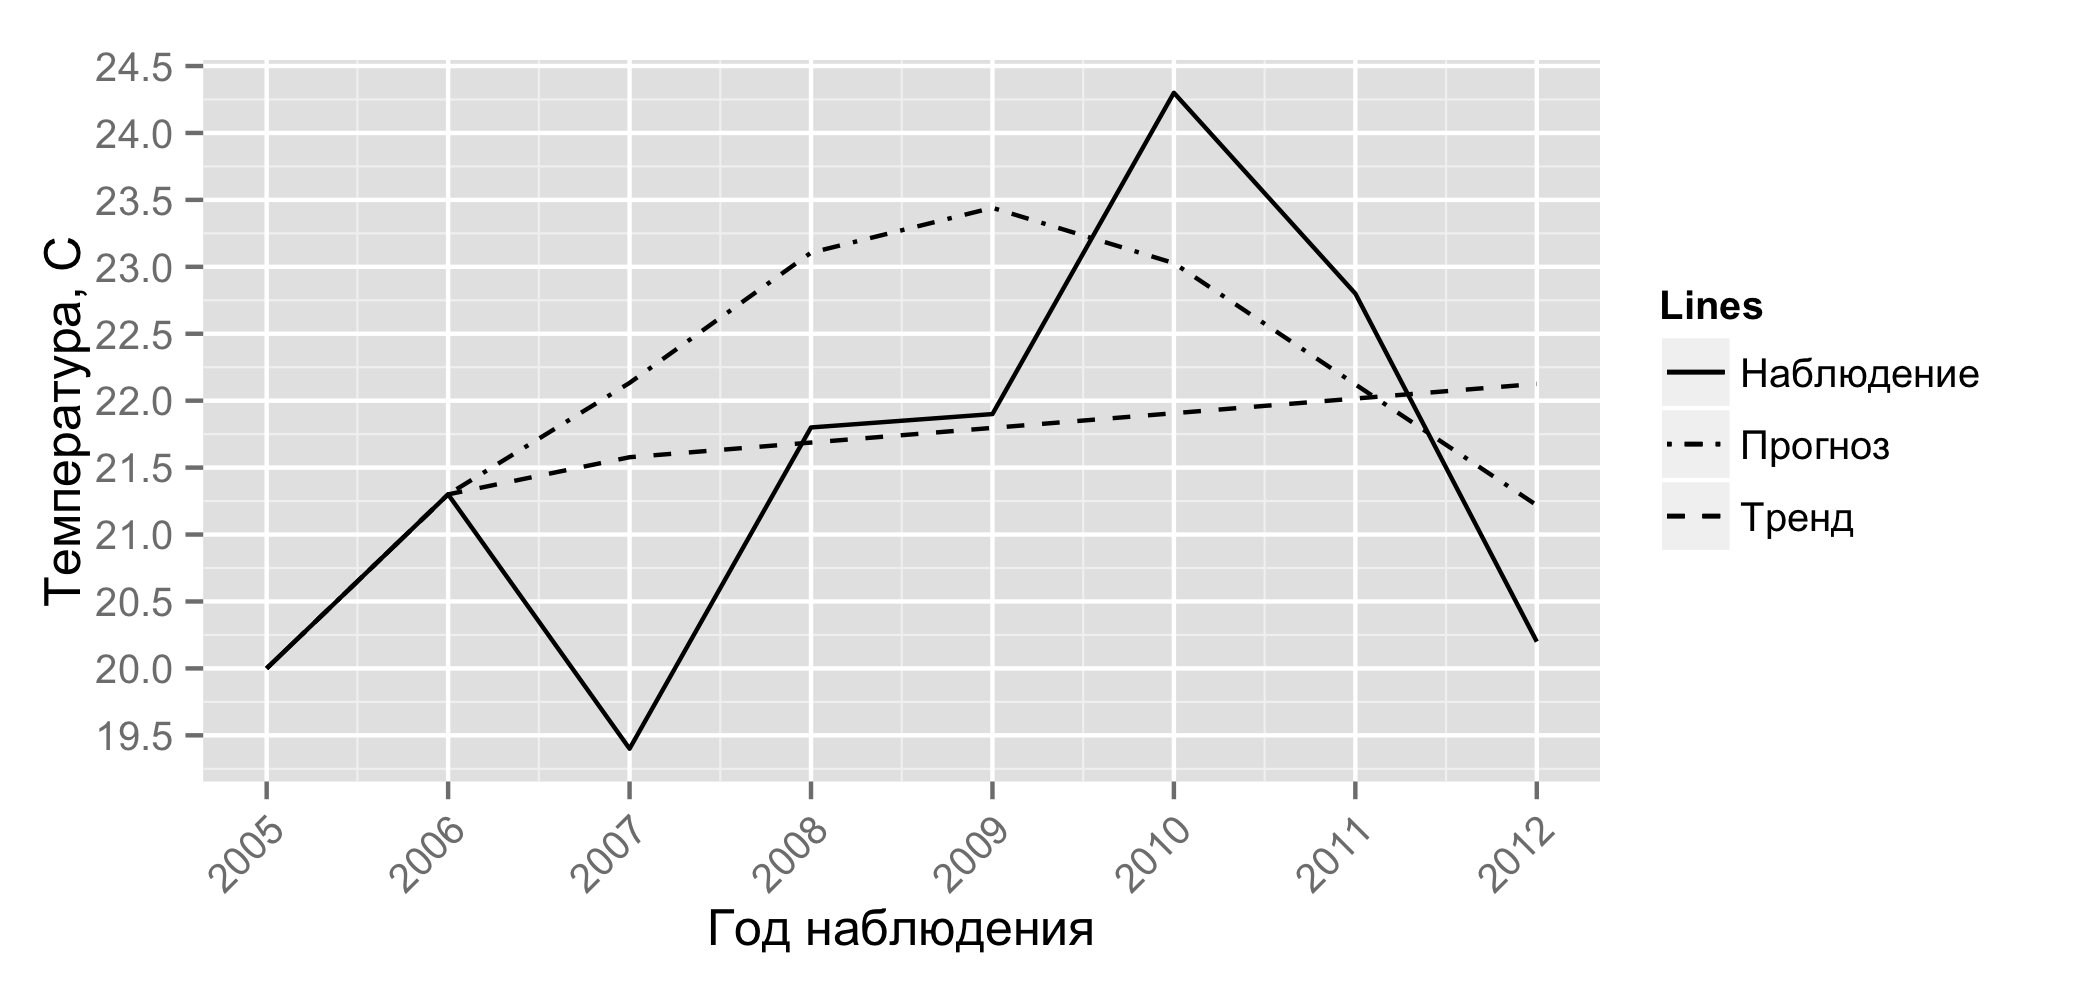
\includegraphics[width=0.9\linewidth]{../../figures/variogram/per-fit-cv-cross-prediction.png}
    \caption{Прогноз по модели $\widehat{\gamma}_6(h)$}
  \end{figure}
  \end{columns}
\end{frame}

\subsection{Автоматический подбор}

\begin{frame}
  \frametitle{Периодическая модель}
  \begin{columns}[c]
  \column{2in}
  Подобранная модель: $ 3.8 + 0.32 \cdot Per(h, 1.3) $
  \column{3in}
   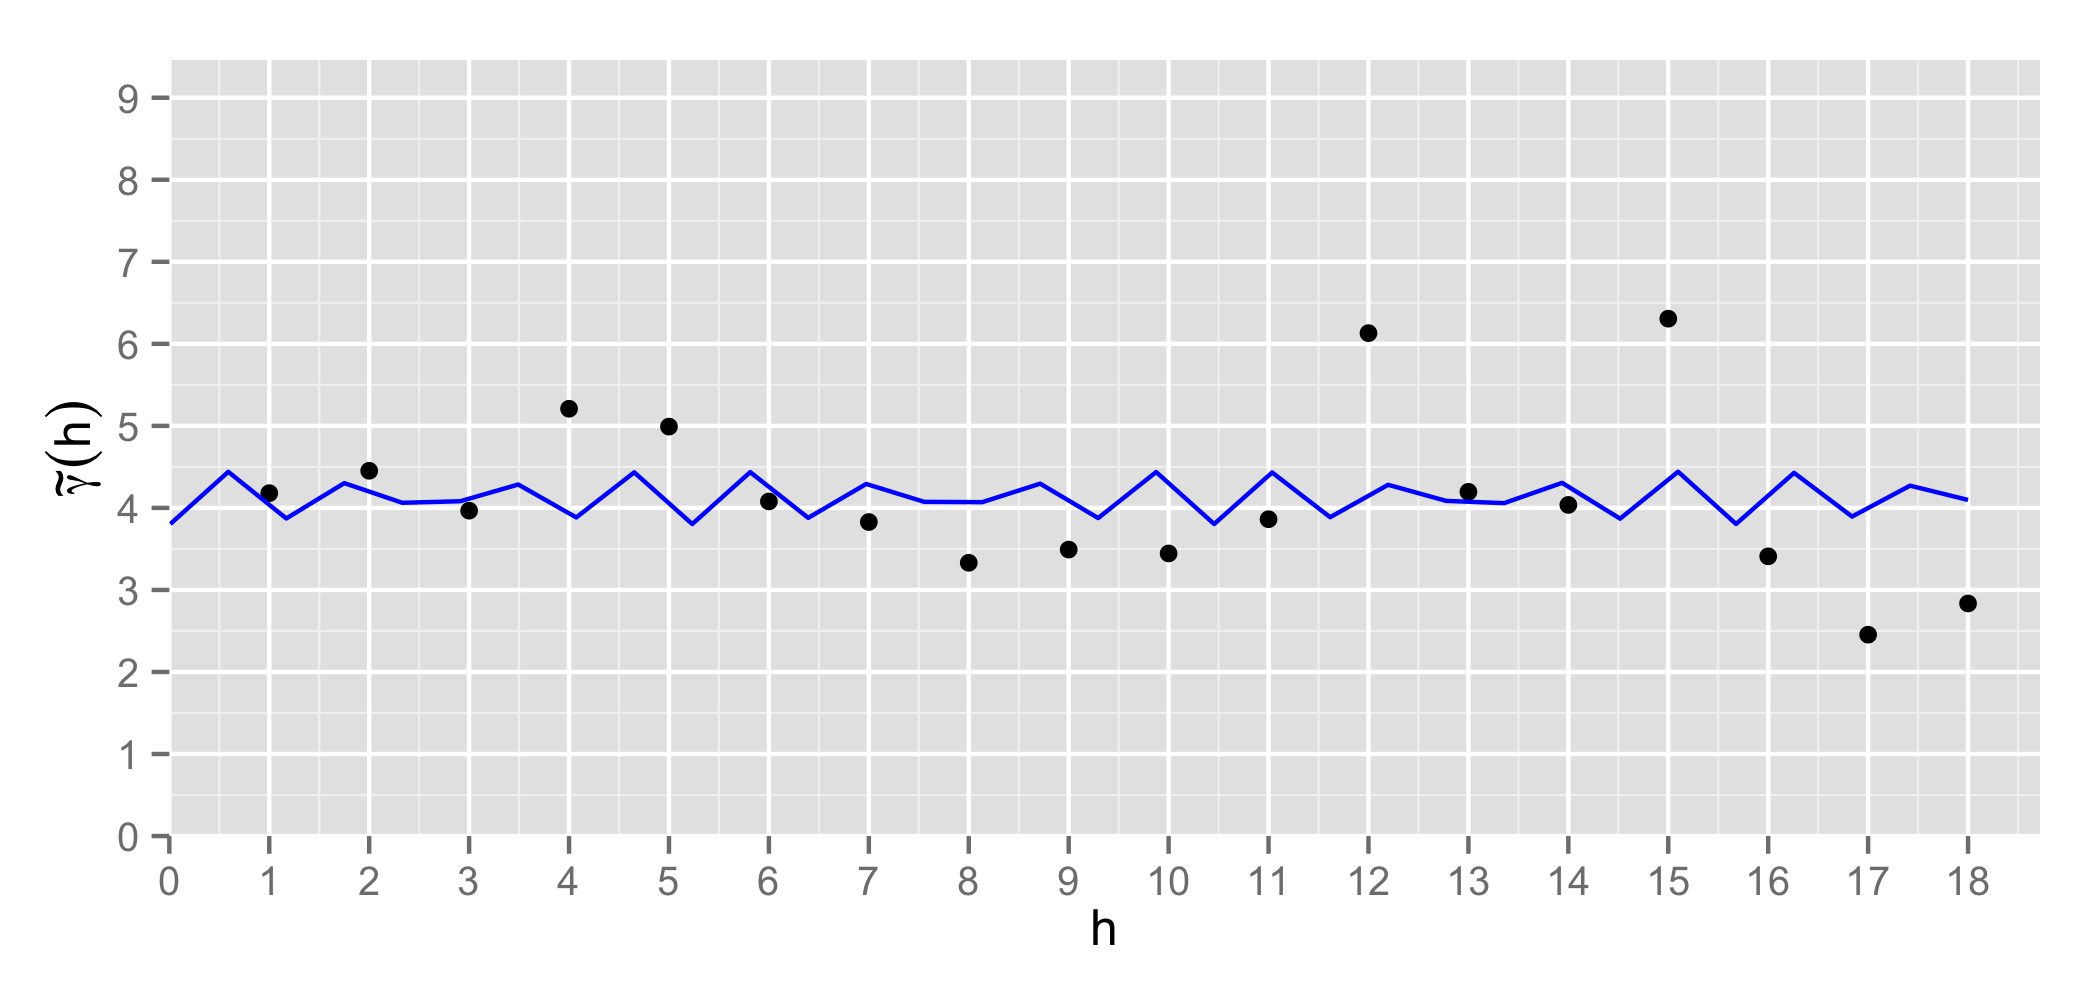
\includegraphics[width=3in]{../../figures/variogram/auto-class-18-modeled.png}
  \end{columns}
\end{frame}

\begin{frame}
  \frametitle{Прогнозирование методом ординарного кригинга}
  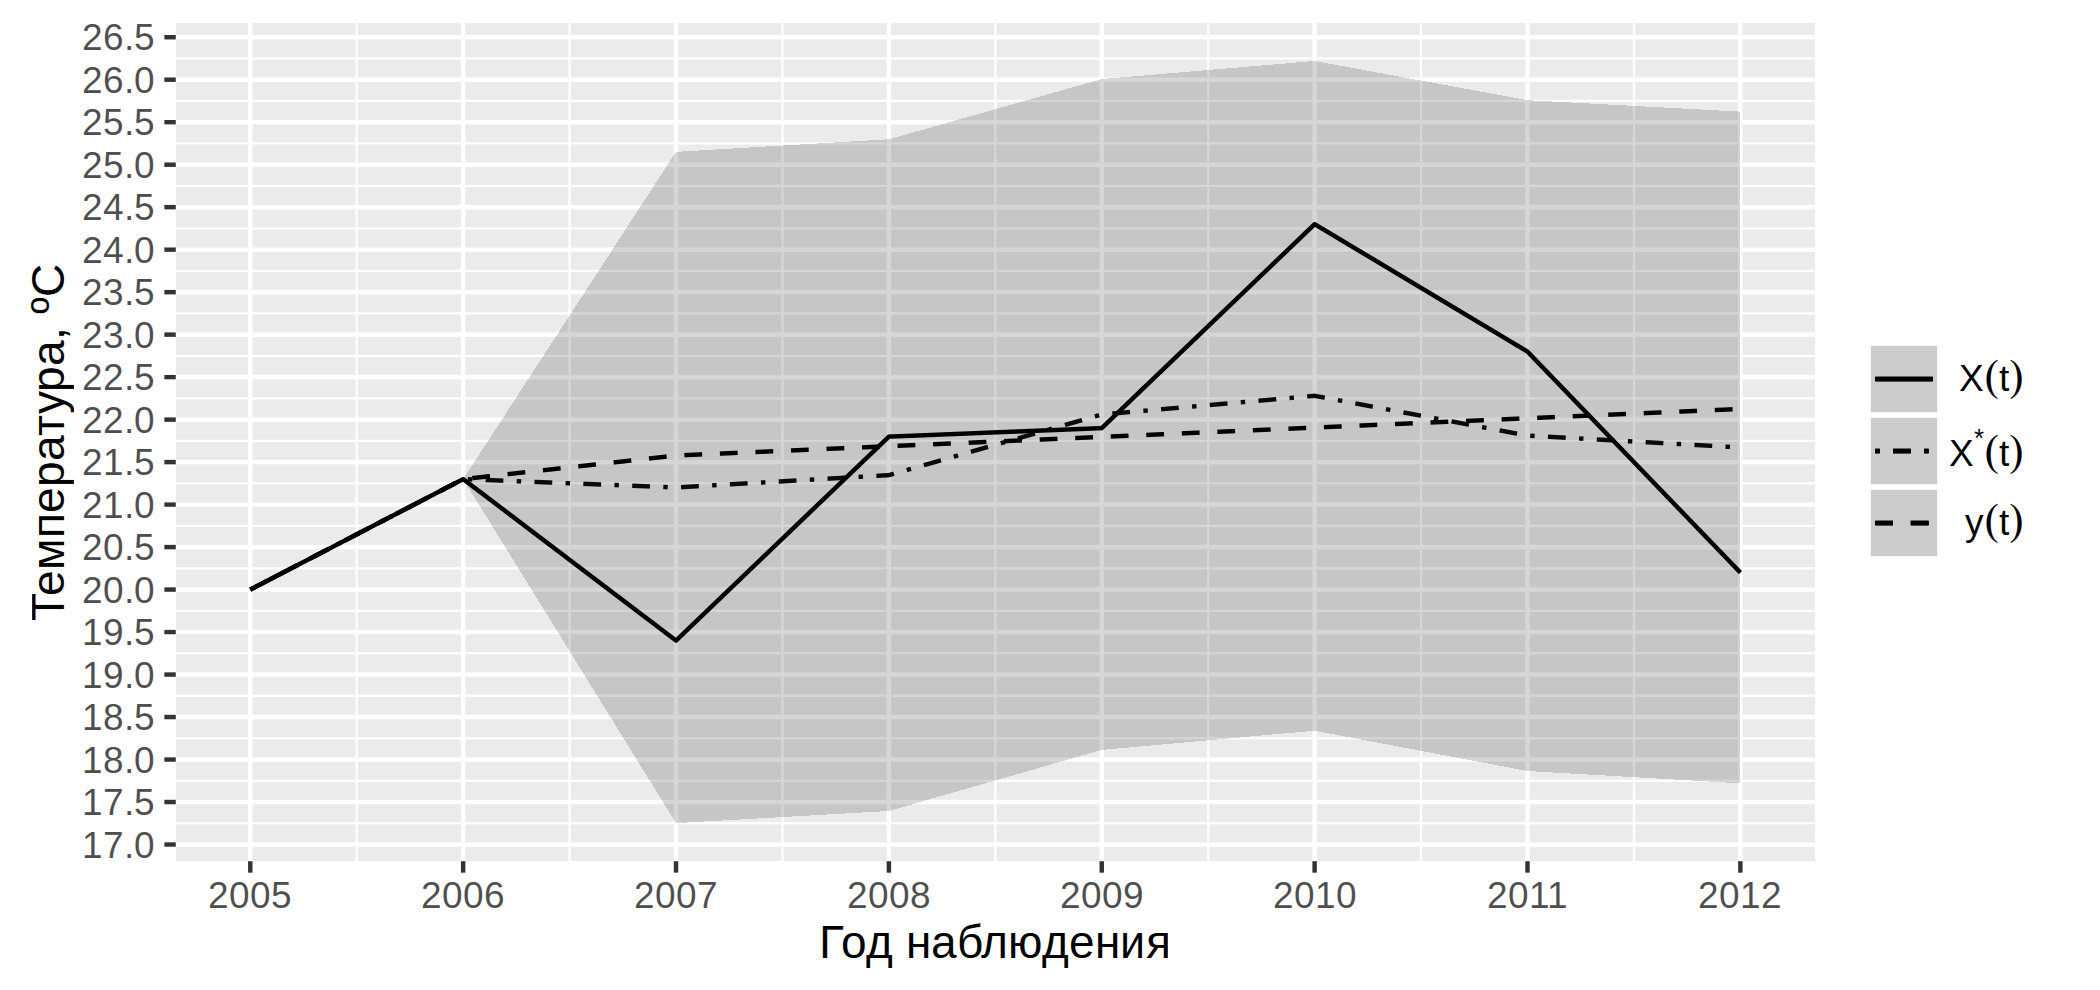
\includegraphics[width=0.95\textwidth]{../../figures/variogram/auto-class-18-cross-prediction.png}
\end{frame}

\begin{frame}
  \frametitle{Волновая модель}
  \begin{columns}[c]
  \column{2in}
  Подобранная модель: $ 4.11 + 1.65 \cdot Wav(h, 3.59) $
  \column{3in}
   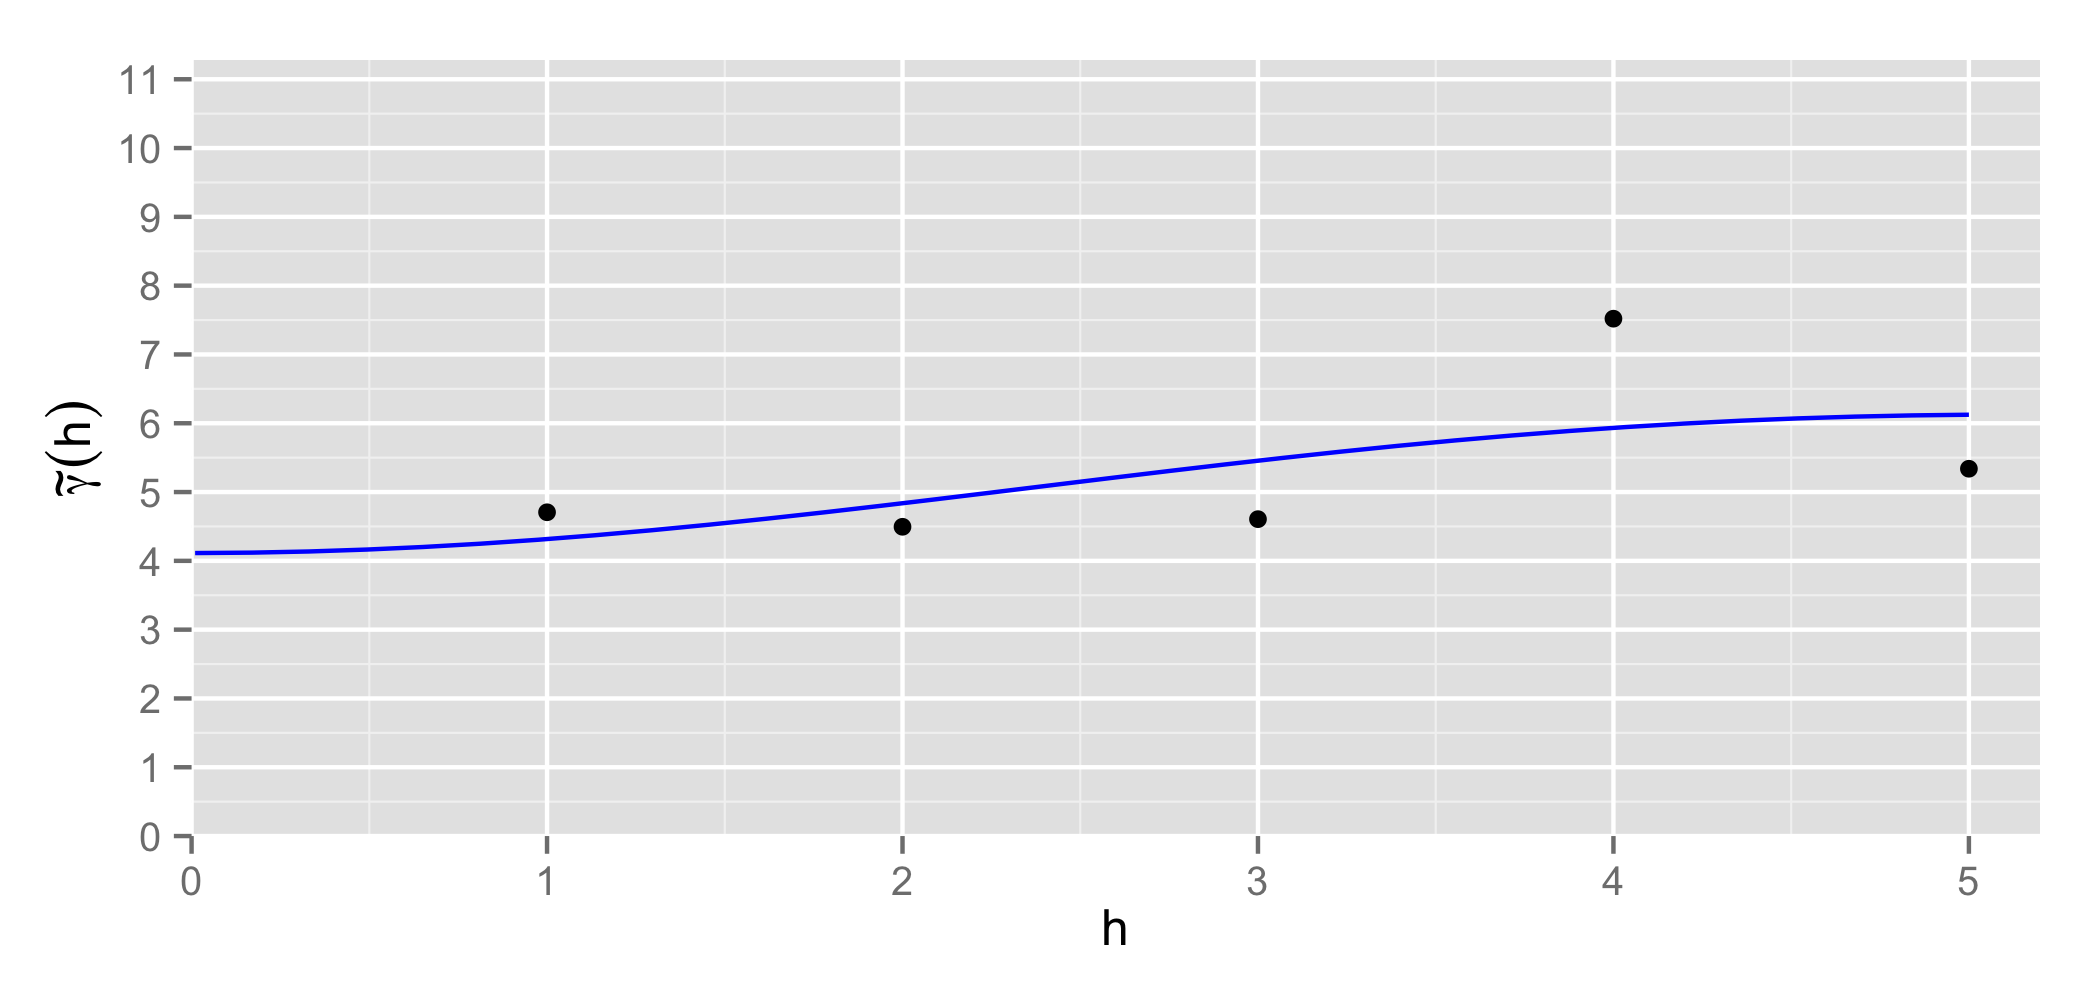
\includegraphics[width=3in]{../../figures/variogram/auto-rob-5-modeled.png}
  \end{columns}
\end{frame}

\begin{frame}
  \frametitle{Прогнозирование методом ординарного кригинга}
  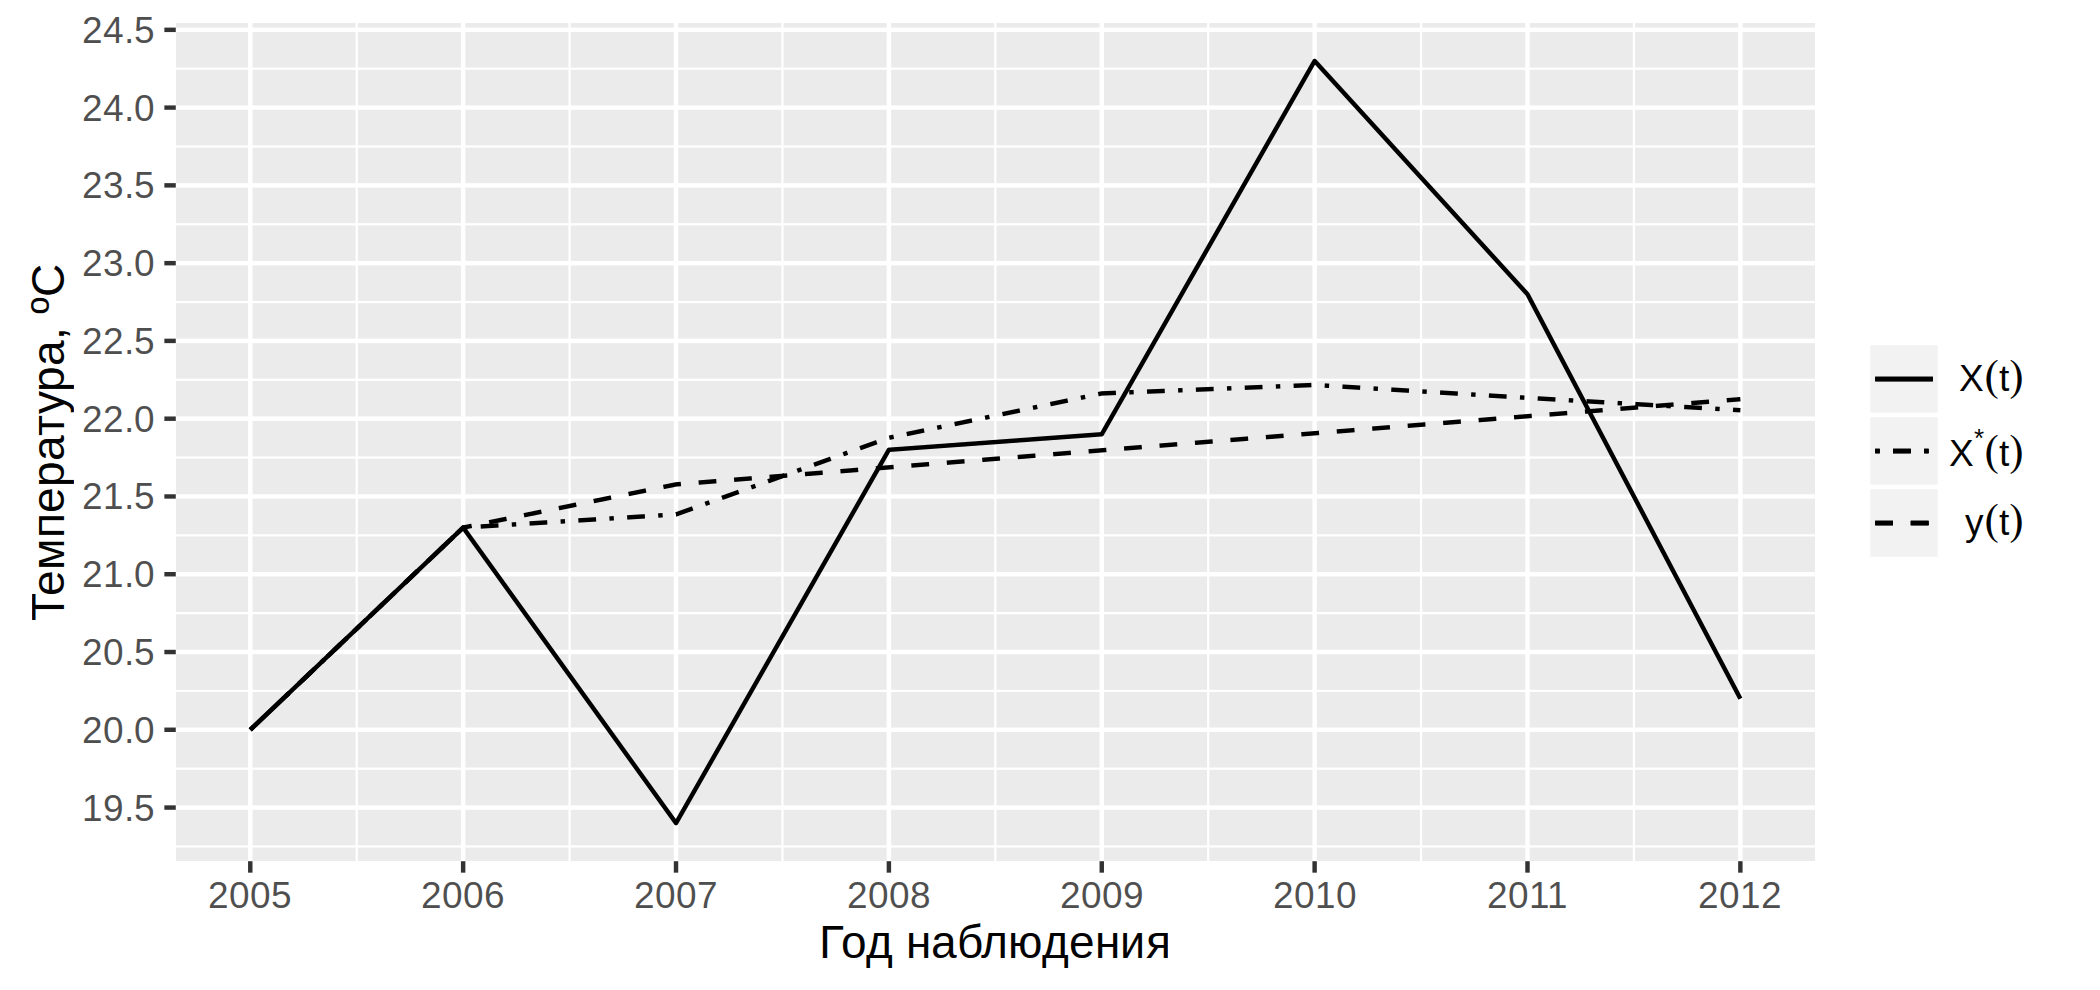
\includegraphics[width=0.95\textwidth]{../../figures/variogram/auto-rob-5-cross-prediction.png}
\end{frame}

\begin{frame}
  \frametitle{Заключение}

\end{frame}

\subsection{}
\begin{frame}
  \frametitle{}
  \begin{center}
    {\Huge Спасибо за внимание!}
  \end{center}
\end{frame}
\end{document}